\documentclass[12pt]{report}
\setcounter{secnumdepth}{5}
\usepackage[french]{babel}
\usepackage{titlesec}
\titleformat{\chapter}[display]
{\normalfont\Huge\bfseries\filcenter}{\chaptertitlename\ \thechapter}{20pt}{\Huge}
\usepackage{geometry}
\geometry{left=2cm, right=2cm, top=2cm, bottom=2cm}
\usepackage{enumitem}
\usepackage{graphicx}
\usepackage{times}
\usepackage{float}
\usepackage{setspace}
\usepackage[T1]{fontenc}
\hyphenpenalty=10000
\exhyphenpenalty=10000
\renewcommand{\thepage}{}
\input{insbox}
\begin{document}
\renewcommand{\thepage}{\arabic{page}}
\setcounter{page}{1}
\thispagestyle{empty}
%page de couverture
\begin{center}
UNIVERSITÉ DE TUNIS EL MANAR\\[15pt]
FACULTÉ DES SCIENCES DE TUNIS

\vspace{20PT}
\begin{figure}[H]
  \centering
  
\includegraphics[scale=0.5]{fst}
\end{figure}
\vspace{20PT}
\begin{huge}
RAPPORT DE STAGE D'ÉTÉ
\end{huge}
\\
\vspace{30pt}
\begin{Large}
Sujet:\\
\end{Large}

\vspace{30pt}
\begin{Huge}
Conception et développement d'une application de gestion des Factures 
\end{Huge}
\\
\vspace{50pt}
\begin{Large}
Réalisé au sein de L'Entreprise Tunisienne d'Activités Pétrolièrs
\end{Large}
\end{center}
\begin{figure}[H]
  \centering
  
\includegraphics[scale=0.5]{etap}
  \label{fig:votre-label}
\end{figure}
\vspace{10pt}
\begin{center}
\begin{Large}
Élaboré par:\\
\vspace{10pt}
SATOURI RANIM\\
\vspace{10pt}
Encadré par:\\
\vspace{10pt}
MANSOURI  AMAL
\end{Large}

\end{center}
\newpage
\thispagestyle{empty}
\textbf{\begin{LARGE}
Remerciement
\end{LARGE}}\\

\fontsize{12}{25}\selectfont
\addcontentsline{toc}{section}{Remerciement}
Tout d’abord, je remercie Dieu de m’avoir accordé la santé et la patience pour mener à bien ce projet.\\

Je souhaite également adresser mes sincères remerciements à l'Entreprise Tunisienne de l'Activité Pétrolière (ETAP) pour m'avoir offert l'opportunité de réaliser ce projet au sein de son organisation. Travailler au sein de l'ETAP a été une expérience enrichissante qui m'a permis de mettre en pratique mes connaissances académiques dans un environnement professionnel stimulant.\\

Je tiens particulièrement à remercier chaleureusement Mme Mansouri Amal, mon encadrante, pour son soutien inestimable, sa passion pour l'enseignement et son encouragement constant tout au long de ce projet. Ses précieux conseils et son expertise ont grandement contribué à l'aboutissement de ce travail.\\


%content

\tableofcontents
\newpage
\listoffigures
\listoftables
\newpage

\section*{\textbf{\begin{LARGE}
Introduction générale
\end{LARGE}}}
\addcontentsline{toc}{section}{Introduction générale}
Dans le monde d'aujourd'hui, l'informatique joue un rôle prépondérant dans le fonctionnement des entreprises. Les applications informatiques ont révolutionné la manière dont les tâches sont accomplies, automatisant des processus complexes et permettant une gestion plus transparente des ressources. \\

L'Entreprise Tunisienne de l'Activité Pétrolière (ETAP) ne fait pas exception à cette tendance. En tant qu'acteur clé du secteur de l'énergie en Tunisie, l'ETAP doit gérer de manière efficace et transparente ses opérations, y compris la gestion des factures d'eau, d'électricité et de gaz .\\

En tant qu'étudiant en génie logiciel à la Faculté des Sciences, j'ai eu l'opportunité de mettre en pratique mes connaissances et compétences en participant à un stage d'initiation au sein de l'Entreprise Tunisienne de l'Activité Pétrolière (ETAP). Ce projet consiste en le développement d'une application de gestion des factures dédiée à l'ETAP. Cette application a été conçue pour répondre spécifiquement aux besoins de l'entreprise et faciliter les tâches de l'administrateur, notamment la gestion, la saisie, le stockage et l'analyse des factures d'eau, d'électricité et de gaz. Elle permet également de suivre des états statistiques qui aident à évaluer la consommation et à prendre les décisions nécessaires.

Le présent rapport se focalise sur la description des différentes étapes de la réalisation de notre sujet. \\
En fait, il est organisé en quatre chapitres :
\begin{itemize}[label={$\rightarrow$}]
	\item \underline{Le premier chapitre :}  << Cadre général du projet >> englobe la présentation de l'entreprise ETAP, la problématique, la solution proposée et enfin la méthodologie de développement.
	\item \underline{Le deuxième chapitre : } << Analyse et spécification des besoins >> souligne les acteurs et les besoins fonctionnels et non fonctionnels de notre projet.
	\item \underline{Le troisième chapitre :} << Architecture et conception de la solution >> décrit l'étude conceptuelle approfondie de l'application.
	\item \underline{Finalement :} << Réalisation de l'application >> dans lequel nous abordons la phase de développement en expliquant les différentes interfaces de l'application, finissant par le chronogramme de travail.
\end{itemize}

\newpage
%les chapitres

\chapter{Cadre Général du projet}
\vspace{100pt}
\begin{center}
Plan du chapitre
\end{center}

\hrule
\vspace{20pt}
Introduction
\begin{enumerate}
	\item Presentation de l'organisme d'accueil
	\item Étude de l'existant
	\item Critique de l'existant
	\item Solutions proposées
	\item Méthodologie de développement
\end{enumerate}

Conclusion
\vspace{20pt}
\hrule
\newpage
\section*{Introduction}
\addcontentsline{toc}{section}{Introduction}
Ce premier chapitre vise à situer le présent projet dans son contexte général. En premier lieu, nous allons donner une présentation détaillée de l'organisme d'accueil, Ensuite, nous allons étudier et critiquer l'existant. Puis, nous allons énoncer la solution proposée et clôturer par la méthodologie de travail adoptée.

\section{Presentation de l'organisme d'accueil}


L'entreprise Tunisienne de l'Activité Pétrolière (ETAP) est une société \mbox{industrielle} et commerciale publique créée en vertu de la loi numero 72-22 du 10 mars 1972, chargée de la gestion des activités pétrolières et d'exploration et de la production de gaz naturel.\\
Elle est classée parmi les entreprises publiques à caractère non administratif (EPNA).
\subsection{Les objectifs de l'ETAP} 

\begin{itemize}[label={$\bullet$}]
    \item Reconstruire la réserve nationale d'hydrocarbures.
    \item Fournir des produits pour le marché pétrolier domestique à des conditions de coûts favorables.
    \item Assurer la formation et le développement des cadres tunisiens dans divers secteurs de l'industrie pétrolière.
    \item Effectuer toutes les recherches liées au pétrole.
    \item Il est possible d'intervenir dans toutes les industries, du commerce, de la finance, du meuble et de l'immobilier directement ou indirectement liées aux hydrocarbures.
	\item Assurer la sécurité de l'approvisionnement en hydrocarbures du pays.
\end{itemize}

\subsection{Les principales activités de l'ETAP}
\begin{itemize}[label={$\bullet$}]
	\item Faites attention à toutes les recherches sur la nature du pétrole.
	\item Vendre du pétrole brut et fournir du gaz naturel au marché local
	\item Exportez du pétrole brut local vers ETAP.
	\item Développer les ressources humaines dans le secteur pétrolier.

\end{itemize}
\subsection{Organisation générale de l'ETAP}
L'ETAP est dirigée par un Président Directeur Général qui représente L'ETAP dans tous les actes civils et administratifs, secondé par un directeur général adjoint et des conseillers. Elle est subdivisée en diverses sections dont cinq directions centrales.
Comme le montre la figure ci-dessous, Mon stage  est réalisé à la direction centrale des ressources plus précisément à la direction informatique.
\begin{figure}[H]
  \centering
  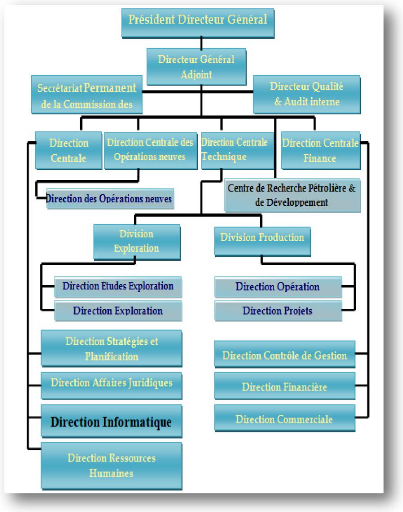
\includegraphics[scale=1]{direction}
  \caption{Organisme de L'ETAP}
  \label{fig:votre-label}
\end{figure}


\subsection{Direction informatique}
L'ETAP a introduit l'outil informatique dès les années 80 dans le but \mbox{principal} de gérer le patrimoine du pays en bandes sismiques.
Le système informatique a également été exploité pour la gestion des applications
relatives aux systèmes d'information ETAP (administrative, comptable, gestion,
application technique, \mbox{financière} et budgétaires ...)
Les principaux projets réalisés au sein de cette \mbox{direction} portent sur :
\begin{itemize}[label={$\bullet$}]
	\item Système d'information
	\item Sécurité informatique
	\item Réseau et application technique d'exploitation
	\item Base de données pétrolière
\end{itemize}



\section{Étude de l'existant}
Afin de comprendre l'application future, il est indispensable de comprendre l'existant et la méthode adoptée pour la gestion des factures.
Auparavant, l'ETAP utilisait principalement des feuilles de calcul Excel pour gérer ses factures. Cela \mbox{signifiait} que les données étaient dispersées et souvent redondantes, ce qui \mbox{compliquait} la recherche et l'analyse des informations.
\section{Critique de l'existant}
Aprés avoir mené une étude approfondie du système actuel,nous avons trouvé diverses critiques:

\begin{itemize}[label={$\bullet$}]
	\item Manque de centralisation des données
	\item Risque de perte de données 
	\item Absence de suivi automatisé 
\end{itemize}

Il est essentiel de souligner que le système existant ne répond pas adéquatement aux besoins en matière de gestion des factures de l'entreprise. Afin de remédier à ces lacunes et de répondre aux besoins croissants de l'entreprise, un nouveau système de gestion des factures est nécessaire.
\section{Solutions proposées}
Face aux limitations du système existant, il est impératif de mettre en place une solution innovante et efficace pour la gestion des factures au sein de l'entreprise. La solution proposée consiste en la conception et la mise en œuvre d'une application de gestion des factures.
La solution proposée présentera les caractéristiques clés suivantes :
\begin{itemize}[label={$\bullet$}]
	\item Interface conviviale : Une interface utilisateur conviviale permettra aux \mbox{utilisateurs} de naviguer facilement dans l'application et d'accéder rapidement aux \mbox{informations} pertinentes.
	\item Centralisation des données : Toutes les données des factures seront \mbox{centralisées} dans une base de données sécurisée, éliminant ainsi la dispersion des \mbox{informations}.
	\item Analyse avancée : L'application offrira des outils d'analyse avancés pour évaluer les coûts des factures par année, ainsi que la consommation d'eau, d'électricité et de gaz par local et par an.
\end{itemize}
\section{Méthodologie de développement}
\subsection{Processus adopté}
Dans un projet informatique, il est indispensable de choisir une bonne démarche pour atteindre les objectifs visés. La réduction du temps, du cout de développement et des risques d'erreurs, sont les soucis majeurs de toutes équipes de développement.\\[9pt]
Pour bien conduire notre projet, nous avons opté pour le Cycle de vie en V. Notre choix s'est basé sur les exigences de ce projet et sur les atouts de ce cycle de vie.\\[9pt]
Le modèle en V est parcouru de gauche à droite suivant la forme de la lettre << V >> dont la branche descendante contient toutes les étapes de la conception du projet, et la branche montante toutes les étapes de tests du projet.\\[9pt]
Le modèle en V demeure actuellement le cycle de vie le plus connu et certainement le plus utilisé. Il permet d'anticiper sur les phases ultérieures de développement du produit.
\begin{figure}[H]
  \centering
  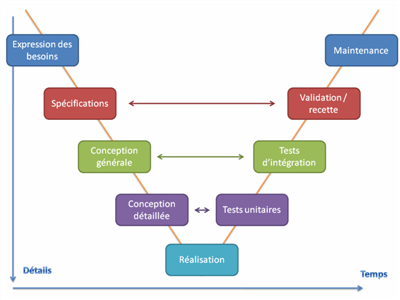
\includegraphics[scale=1]{v}
  \caption{Représentation de la méthodologie cycle en V}
  \label{fig:votre-label}
\end{figure}
\subsection{Language de modélisation}
Après le choix de la méthodologie, nous avons besoin d'un langage de modélisation unifiée pour la modélisation de notre projet dans le but de maîtriser sa complexité et d'assurer sa cohérence. Afin de concevoir notre système, nous avons choisi l'UML (Unified Modeling Language) comme un langage de modélisation.\\[9pt]
Ce choix est basé sur les points forts de ce langage qui est standard et offre la possibilité de schématiser graphiquement des systèmes complexes sous un format simplifié et normalisé. \\[9pt]
L'UML propose divers diagrammes de modélisations, parmi lesquelles, ceux que nous allons utiliser sont :
\begin{itemize}[label={$\surd$}]
	\item \textbf{Le diagramme de cas d'utilisation} qui est un diagramme fonctionnel, il permet de représenter les interactions entre les utilisateurs et le système\\
	\item \textbf{Le diagramme de classes} qui est un diagramme statique, il permet de représenter les éléments du système (classes et packages), leur contenu (attributs et méthodes) ainsi que les associations qui les relient.
	\item \textbf{Le diagramme de séquence} qui est un diagramme dynamique, il permet de représenter temporellement l'échange entre l'utlisateur et le système.
\end{itemize}

\section*{Conclusion}
\addcontentsline{toc}{section}{Conclusion}
Ce premier chapitre nous a permis de mettre le projet dans son cadre général en présentant l'organisme d'accueil l'ETAP, l'étude et la critique de l'existant ainsi qu'une analyse et description de la méthodologie de développement qui seront utilisés dans ce projet.\\[9pt]
Maintenant nous sommes en mesure d'entamer notre deuxième chapitre qui est l'analyse et la spécification des besoins.
%chapitre 2
\chapter{Analyse et spécification des besoins}
\vspace{100pt}
\begin{center}
Plan du chapitre
\end{center}

\hrule
\vspace{20pt}
Introduction
\begin{enumerate}
	\item Identification des acteurs
	\item Identification des besoins
	\item Diagramme des cas d'utilisation global
\end{enumerate}

Conclusion
\vspace{20pt}
\hrule
\newpage

\section*{Introduction}
\addcontentsline{toc}{section}{Introduction}
L'analyse et la spécification des besoins représentent une phase primordiale dans la méthodologie de travail adopté, à savoir le cycle de vie en V. En outre, les exigences définies dans ce chapitre sont les fonctionnalités que nous envisageons à implémenter dans l'application. En premier lieu, nous allons identifier les acteurs du système. Ensuite, nous allons présenter les besoins de ce projet. Puis, nous allons clôturer par spécifier les besoins.

\section{Identification des acteurs}
Un acteur est la personne ou le logiciel qui interagit avec notre système afin de répondre à un besoin bien déterminé.\\
Dans notre application, nous avons identifié essentiellement deux acteurs à savoir l'Administrateur et l'Employé:

\begin{itemize}[label={$\bullet$}]
	\item L'Admin : c'est la personne qui gère les tâches administratives, à savoir gérer les employés ,les factures.
	\item L'employé : C'est la personne qui a le droit d'ajouter et de consulter les factures
\end{itemize}
\section{Identification des besoins}
L'identification des besoins consiste à traduire les objectifs du projet en un ensemble de besoins fonctionnels et non fonctionnels. 
\subsection{Les besoins fonctionnels}
Dans cette partie, nous présentons les différents besoins fonctionnels que notre système doit répondre.\\
Administrateur:
\begin{itemize}[label={$\bullet$}]
	\item S'authentifier : L'administrateur est capable d'accéder aux fonctionnalités de l'application en se connectant.
	\item Gérer les Employés : Consulter , Ajouter, supprimer et modifier les informations des Employés.
	\item Gérer les factures : Consulter , Ajouter, supprimer et modifier les Factures.
	\item Suivre les états statistiques 
\end{itemize}
\vspace{10pt}
L'Employé :
\begin{itemize}[label={$\bullet$}]
	\item S'authentifier : L'employé est capable d'accéder aux fonctionnalités de l'application en se connectant.
	\item Gérer les factures : Consulter et Ajouter les Factures.
	\item Suivre les états statistiques 
\end{itemize}

\subsection{Les besoins non fonctionnels}
\begin{itemize}[label={$\bullet$}]
	\item L'ergonomie : l'application doit fournir des interfaces simples, conviviales et bien structurées afin que l'utilisateur puisse l'exploiter sans aucunes difficultés.
	\item L'extensibilité : le code doit être clair et le système doit être conforme à une architecture évolutive pour permettre de renouveler ou encore ajouter des nouvelles fonctionnalités.
	\item Besoins de sécurité : l'application doit être hautement sécurisé ,tout accès doit être protégé par un mot de passe et un privilège d'accès.
\end{itemize}
\section{Spécification des besoins}
Dans cette partie, nous spécifions en détail les besoins fonctionnels de notre système d'une manière formelle en utilisant le diagramme de cas d'utilisation du langage de modélisation UML et des descriptions textuelles.
\subsection{Diagramme de cas d'utilisation global}
Le diagramme de cas d'utilisation général nous donne une vision globale sur l'application en identifiant les acteurs et en structurant les besoins fonctionnels relatifs à l'application.
\\
La figure 2.1 illustre le diagramme de cas d'utilisation global de notre application.

\begin{figure}[H]
  \centering
  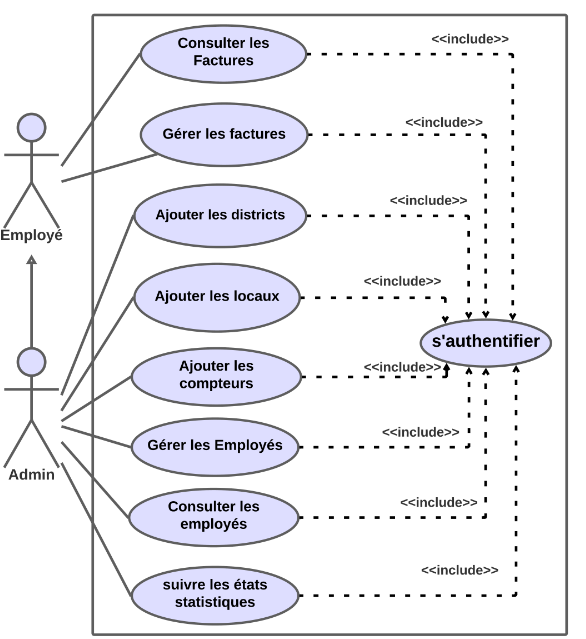
\includegraphics[width=18cm,height=17cm]{newauth3}
  \caption{Diagramme de cas d'utilisation global}
  \label{fig:votre-label}
\end{figure}
\subsection{Raffinement et descriptions textuelles des cas d'utilisation}
Dans ce qui suit, nous allons raffiner quelques cas d'utilisation qu'on juge prioritaires et les décrire par des descriptions textuelles.
\\
Nous allons commencer par une description textuelle du cas d'utilisation << S'authetifier >> représenté par le tableau 2.1.
%table
\begin{table}[H]
\centering

\def\arraystretch{1.3}
\begin{tabular}{|p{2.5cm}|p{14.5cm}|}
   
   \hline
   \multicolumn{2}{|c|}{
   \textbf{SOMMAIRE D'IDENTIFICATION}
   } \\
   \hline
   \textbf{Titre}  &  S'authentifier \\
   \hline
   \textbf{Objectif} &  Permet aux utilisateurs de s'authentifier sur l'application  \\
   \hline
    \textbf{Acteurs}  &  Administrateur,Employé \\
   \hline
   \multicolumn{2}{|c|}{ \textbf{DESCRIPTION DES ENCHAINEMENTS} } \\
   \hline
   \multicolumn{2}{|p{17cm}|}{\textbf{ précondition : }
   \begin{itemize}[label={$\bullet$}]
      \item  l'utilisateur n'est pas authentifié sur l'application 
   \end{itemize}} \\
   \hline
   \multicolumn{2}{|p{17cm}|}{\textbf{ Scénario nominal : }
   \begin{enumerate}
      \item Le système affiche le formulaire de connection.
      \item  L'utilisateur saisit son identifiant et son mot de passe.
      \item  L'utilisateur clique sur le bouton  << Se Connecter >>.
      \item  L'utilisateur accède à la page d'accueil .
   \end{enumerate}} \\
   \hline
   \multicolumn{2}{|p{17cm}|}{\textbf{ Scénario alternatif : }
   \begin{itemize}[label={$\bullet$}]
      \item  Si l'identifiant et/ou le mot de passe sont manquants ou invalides , le système affiche un message d'erreur.      
   \end{itemize}} \\
   \hline
   \multicolumn{2}{|p{17cm}|}{\textbf{ Post condition : }
   \begin{itemize}[label={$\bullet$}]
      \item L'utilisateur est authentifié et redirigé vers la page d'accueil.
   \end{itemize}} \\
   \hline
\end{tabular}
\caption{Description textuelle du cas d'utilisation << S'authetifier >>}
\end{table}
%end table
Le raffinement du cas d'utilisation << Gérer les Factures >> est representé par la figure 2.2

\begin{figure}[H]
  \centering
  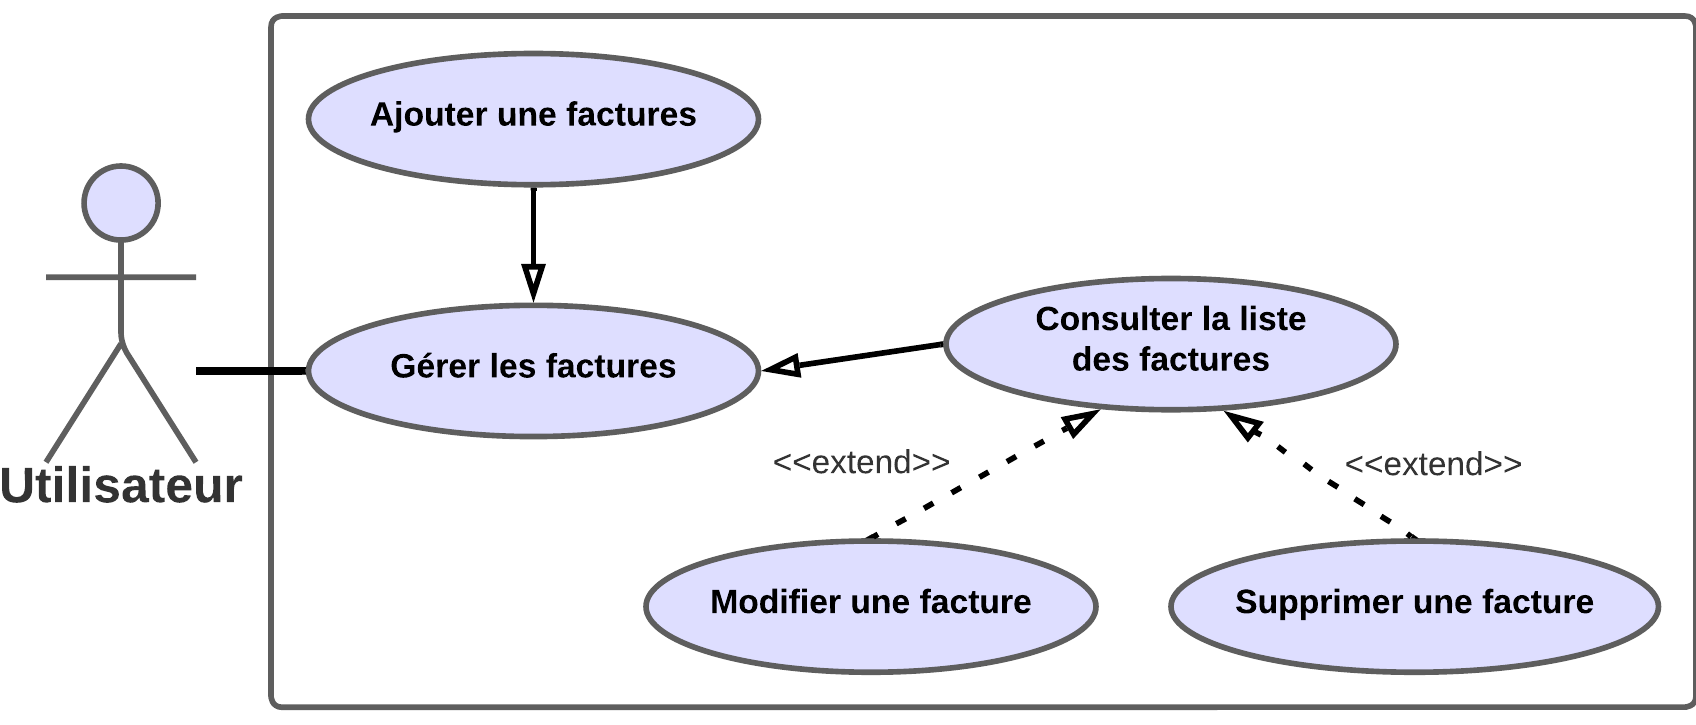
\includegraphics[width=15cm,height=5cm]{gererfact}
  \caption{raffinement du cas d'utilisation << Gérer les Factures >> }
  \label{fig:votre-label}
\end{figure}
Le raffinement du cas d'utilisation << Gérer les Employés >> est representé par la figure 2.3

\begin{figure}[H]
  \centering
  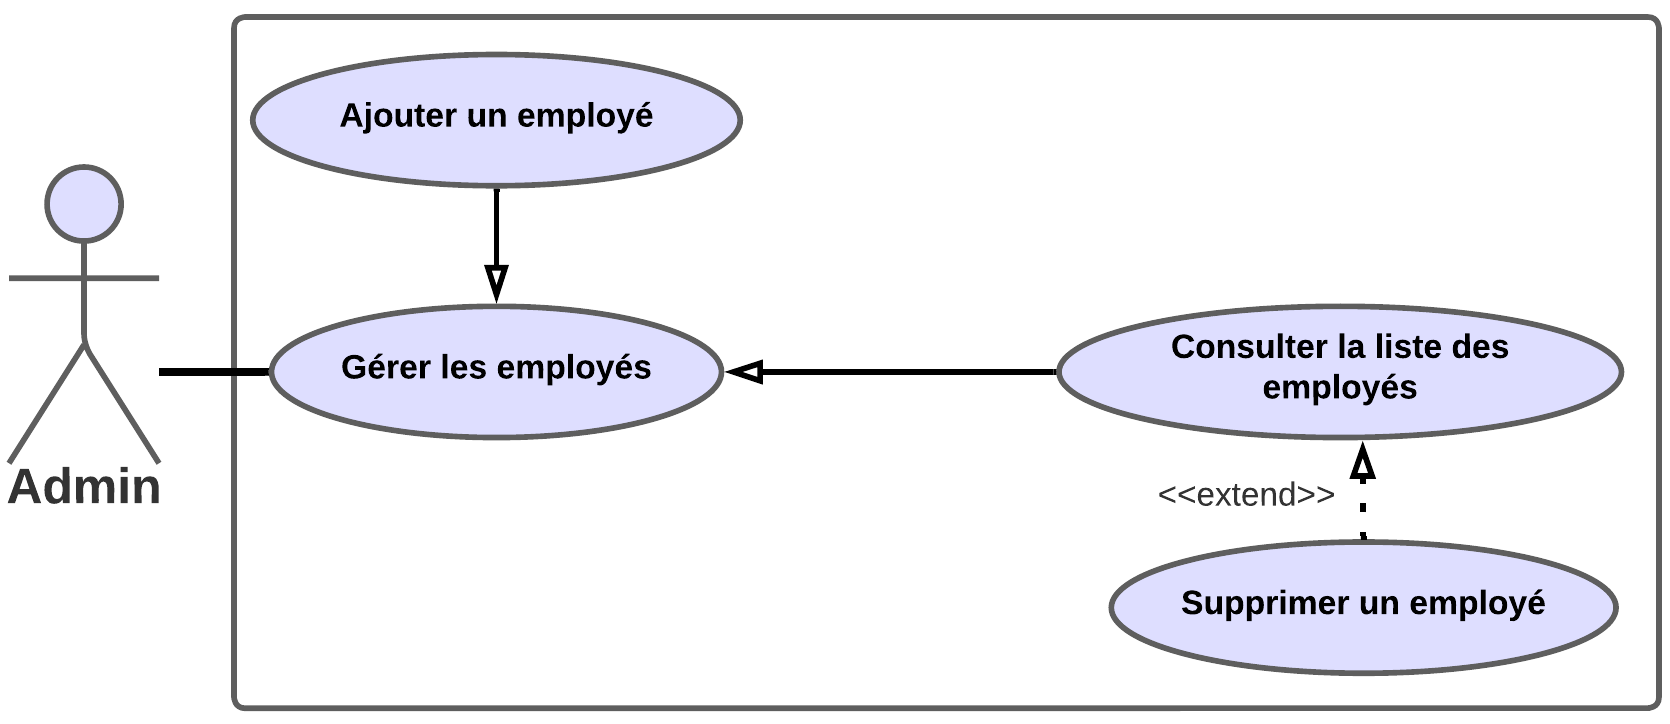
\includegraphics[width=15cm,height=5cm]{gereremp}
  \caption{raffinement du cas d'utilisation << Gérer les Employés >> }
  \label{fig:votre-label}
\end{figure}
%table 3
\begin{table}[H]
\centering
\def\arraystretch{1.5}
\begin{tabular}{|p{2.5cm}|p{14.5cm}|}
   \hline
   \multicolumn{2}{|c|}{
   \textbf{SOMMAIRE D'IDENTIFICATION}
   } \\
   \hline
    \textbf{Titre} &  Supprimer un Employé  \\
   \hline
    \textbf{Objectif}  &  Permet à l'administrateur de Supprimer un Employé de l'application .  \\
   \hline
    \textbf{Acteurs}  &  Administrateur \\
   \hline
   \multicolumn{2}{|c|}{ \textbf{DESCRIPTION DES ENCHAINEMENTS} } \\
   \hline
   \multicolumn{2}{|p{17cm}|}{\textbf{ précondition : }
   \begin{itemize}[label={$\bullet$}]
      \item L'administrateur est authentifié sur l'application. 
      \item   Il y a au moins un Employé ajouté. 
   \end{itemize}} \\
   \hline
   \multicolumn{2}{|p{17cm}|}{\textbf{ Scénario nominal : }
   \begin{enumerate}
      \item  L'administrateur clique sur le bouton << Consulter les Employé >> .
      \item  Le système retourne la liste d'employés.
      \item  L'administrateur choisit un Employé et clique sur le bouton << Supprimer >> .
      \item  Le système retourne une boite de confirmation.
      \item  L'administrateur confirme la supression.
      \item  Le système affiche un message indiquant le succès de l'opération.
      
   \end{enumerate}} \\
   \hline
   \multicolumn{2}{|p{17cm}|}{\textbf{ Scénario alternatif : }
   \begin{itemize}[label={$\bullet$}]
      \item  L'administarteur annule la supression de l'employé.   
   \end{itemize}} \\
   \hline
   \multicolumn{2}{|p{17cm}|}{\textbf{ Post condition : }
   \begin{itemize}[label={$\bullet$}]
      \item  L'employé choisi est supprimé.
   \end{itemize}} \\
   \hline
\end{tabular}
\caption{Description textuelle du cas d'utilisation << Supprimer un Utilisateur >>}
\end{table}
%table2
\begin{table}[H]
\centering
\def\arraystretch{2}
\begin{tabular}{|p{2.5cm}|p{14.5cm}|}
   \hline
   \multicolumn{2}{|c|}{
   \textbf{SOMMAIRE D'IDENTIFICATION}
   } \\
   \hline
    \textbf{Titre}  &  Modifier une Facture  \\
   \hline
   \textbf{Objectif}  &  Permet à l'utilisateur de modifier une facture.  \\
   \hline
    \textbf{Acteurs}  &  Administrateur,Employé\\
   \hline
   \multicolumn{2}{|c|}{\textbf{DESCRIPTION DES ENCHAINEMENTS} } \\
   \hline
   \multicolumn{2}{|p{17cm}|}{\textbf{ précondition : }
   \begin{itemize}[label={$\bullet$}]
      \item  L'utilisateur est authentifié sur l'application. 
      \item   Il y a au moins une facture ajoutée. 
   \end{itemize}} \\
   \hline
   \multicolumn{2}{|p{17cm}|}{\textbf{ Scénario nominal : }
   \begin{enumerate}
      \item  L'utilisateur clique sur le bouton << Consulter les Factures >> .
      \item  Le système retourne la liste des factures.
      \item  L'utilisateur choisit une facture et clique sur le bouton << Modifier >> .
      \item  Le système Retourne un formulaire remplit des données de la facture choisit. 
      \item  L'utilisateur modifie les données .
      \item  L'utilisateur clique sur le bouton << Modifier >>.
      \item  Le système retourne une boite de confirmation.
      \item  L'utilisateur confirme la supression.
      \item  Le système affiche un message indiquant le succès de l'opération.
      
   \end{enumerate}} \\
   \hline
   \multicolumn{2}{|p{17cm}|}{\textbf{Scénario alternatif : }
   \begin{itemize}[label={$\bullet$}]
      \item  Le système affiche un message d'erreur si les  informations entrées sont manquants ou erronées.     
   \end{itemize}} \\
   \hline
   \multicolumn{2}{|p{17cm}|}{\textbf{ Post condition : }
   \begin{itemize}[label={$\bullet$}]
      \item  La facture est Modifié.
   \end{itemize}} \\
   \hline
\end{tabular}
\caption{Description textuelle du cas d'utilisation << Modifier une Facture >>}
\end{table}
%end second table


%table 4
\begin{table}[H]
\centering
\def\arraystretch{1.5}
\begin{tabular}{|p{2.5cm}|p{14.5cm}|}
   \hline
   \multicolumn{2}{|c|}{
   \textbf{SOMMAIRE D'IDENTIFICATION}
   } \\
   \hline
    \textbf{Titre}  &    Ajouter un compteur \ \\
   \hline
   \textbf{Objectif}  & Permet à l'administrateur d'Ajouter un compteur .  \\
   \hline
    \textbf{Acteurs}  &  Administrateur\\
   \hline
   \multicolumn{2}{|c|}{ \textbf{DESCRIPTION DES ENCHAINEMENTS} } \\
   \hline
   \multicolumn{2}{|p{17cm}|}{\textbf{ précondition : }
   \begin{itemize}[label={$\bullet$}]
      \item  L'administrateur est authentifié sur l'application. 
      \item   Il y a au moins un District et un Local ajouté. 
   \end{itemize}} \\
   \hline
   \multicolumn{2}{|p{17cm}|}{\textbf{ Scénario nominal : }
   \begin{enumerate}
      \item  L'administrateur clique sur le bouton << Ajouter un compteur >> .
      \item  Le système retourne un formulaire  .
      \item  L'administrateur choisit le District et le local a partir du menu déroulant.
      \item  L'administrateur choisit  le type de compteur.
      \item  L'administrateur saisit la référence du compteur et clique sur le bouton << Ajouter >>.
      \item Le système affiche un message indiquant le succès de l'opération.
      
   \end{enumerate}} \\
   \hline
   \multicolumn{2}{|p{17cm}|}{\textbf{ Scénario alternatif : }
   \begin{itemize}[label={$\bullet$}]
      \item  Le système affiche un message d'erreur si les  informations entrées sont manquants ou erronées.     
   \end{itemize}} \\
   \hline
   \multicolumn{2}{|p{17cm}|}{\textbf{ Post condition : }
   \begin{itemize}[label={$\bullet$}]
      \item  Le compteur est ajouté.
   \end{itemize}} \\
   \hline
\end{tabular}
\caption{Description textuelle du cas d'utilisation << Ajouter un compteur >>}
\end{table}


\section*{Conclusion}
\addcontentsline{toc}{section}{Conclusion}
Le travail réalisé dans ce chapitre nous a conduits à construire une meilleure vision de la solution puisque nous avons dégagé les acteurs, identifié les besoins fonctionnels et non fonctionnels et décrit la spécification technique de notre projet.
\\
Le chapitre suivant sera consacré à l'étude conceptuelle de notre application.

%chapitre 3
\chapter{Architecture et Conception de la solution}
\vspace{100pt}
\begin{center}
Plan du chapitre
\end{center}

\hrule
\vspace{20pt}
Introduction
\begin{enumerate}
	\item Architecture de L'application
	\item Conception
\end{enumerate}

Conclusion
\vspace{20pt}
\hrule
\newpage
\newpage
\section*{Introduction}
\addcontentsline{toc}{section}{Introduction}
La conception est une étape très importante dans la réalisation de notre application, elle permet de concevoir la base de données de notre futur système d'information pour réduire la complexité et lever les ambiguïtés. De plus, elle peut acquérir une meilleure compréhension du système et ainsi gagner du temps.\\
En premier lieu, nous allons décrire l'architecture de notre application. Ensuite, nous allons nous intéresser à la conception du système.
\section{Architecture de L'application}
La conception de l'architecture logicielle représente une étape primordiale dans le processus de conception .Elle dépend de plusieurs facteurs et aide à réaliser les besoins non fonctionnels de l'application comme l'extensibilité et l'évolutivité.\\
Dans le cadre de ce projet, on a choisi une architecture 1-tier pour développer une application bureau.

 Cette architecture est également appelée « client lourd » ou « monolithique ». Dans cette approche, l'intégralité de l'application réside et s'exécute localement sur l'ordinateur de l'utilisateur.\\  L'interface utilisateur, le logique métier et l'accès à la base de données MySQL sont tous inclus dans un code source unique. Cela signifie que notre application bureau est une entité autonome qui gère toutes les fonctionnalités sans dépendre de composants de serveur externes.
\begin{figure}[H]
  \centering
  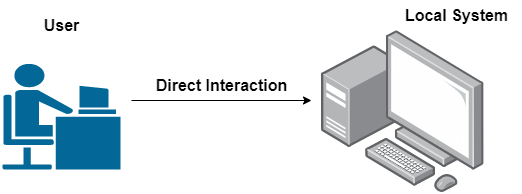
\includegraphics[width=18.5cm]{1tier}
  \caption{Architecture Logicielle de l'application }
  \label{fig:votre-label}
\end{figure}
 L’avantage de cette architecture est sa simplicité car elle ne nécessite pas la mise en place de serveurs ou services supplémentaires. 
 \\
 Cependant, il peut présenter des limites en termes de maintenabilité et d’évolutivité à mesure que l’application se développe.
 
Cette architecture est adaptée aux applications de bureau autonome, où les utilisateurs exécutent l'application localement et n'ont pas besoin d'un accès à distance aux données ou à la logique de l'application.
\section{Conception}

\subsection{Vue dynamique}
Le diagramme de séquence est un diagramme qui décrit l'aspect dynamique du systéme, il permet de représenter, de façon séquentielle, l'échange entre des acteurs du système et des instances de classes, de composants et de sous-systèmes.
\\
Nous allons présenter ci-après les diagrammes de séquences, que nous avons jugés importants pour la réalisation de notre application.\subsubsection{Diagramme de séquence << Authentification >>}

\begin{figure}[H]
  \centering
  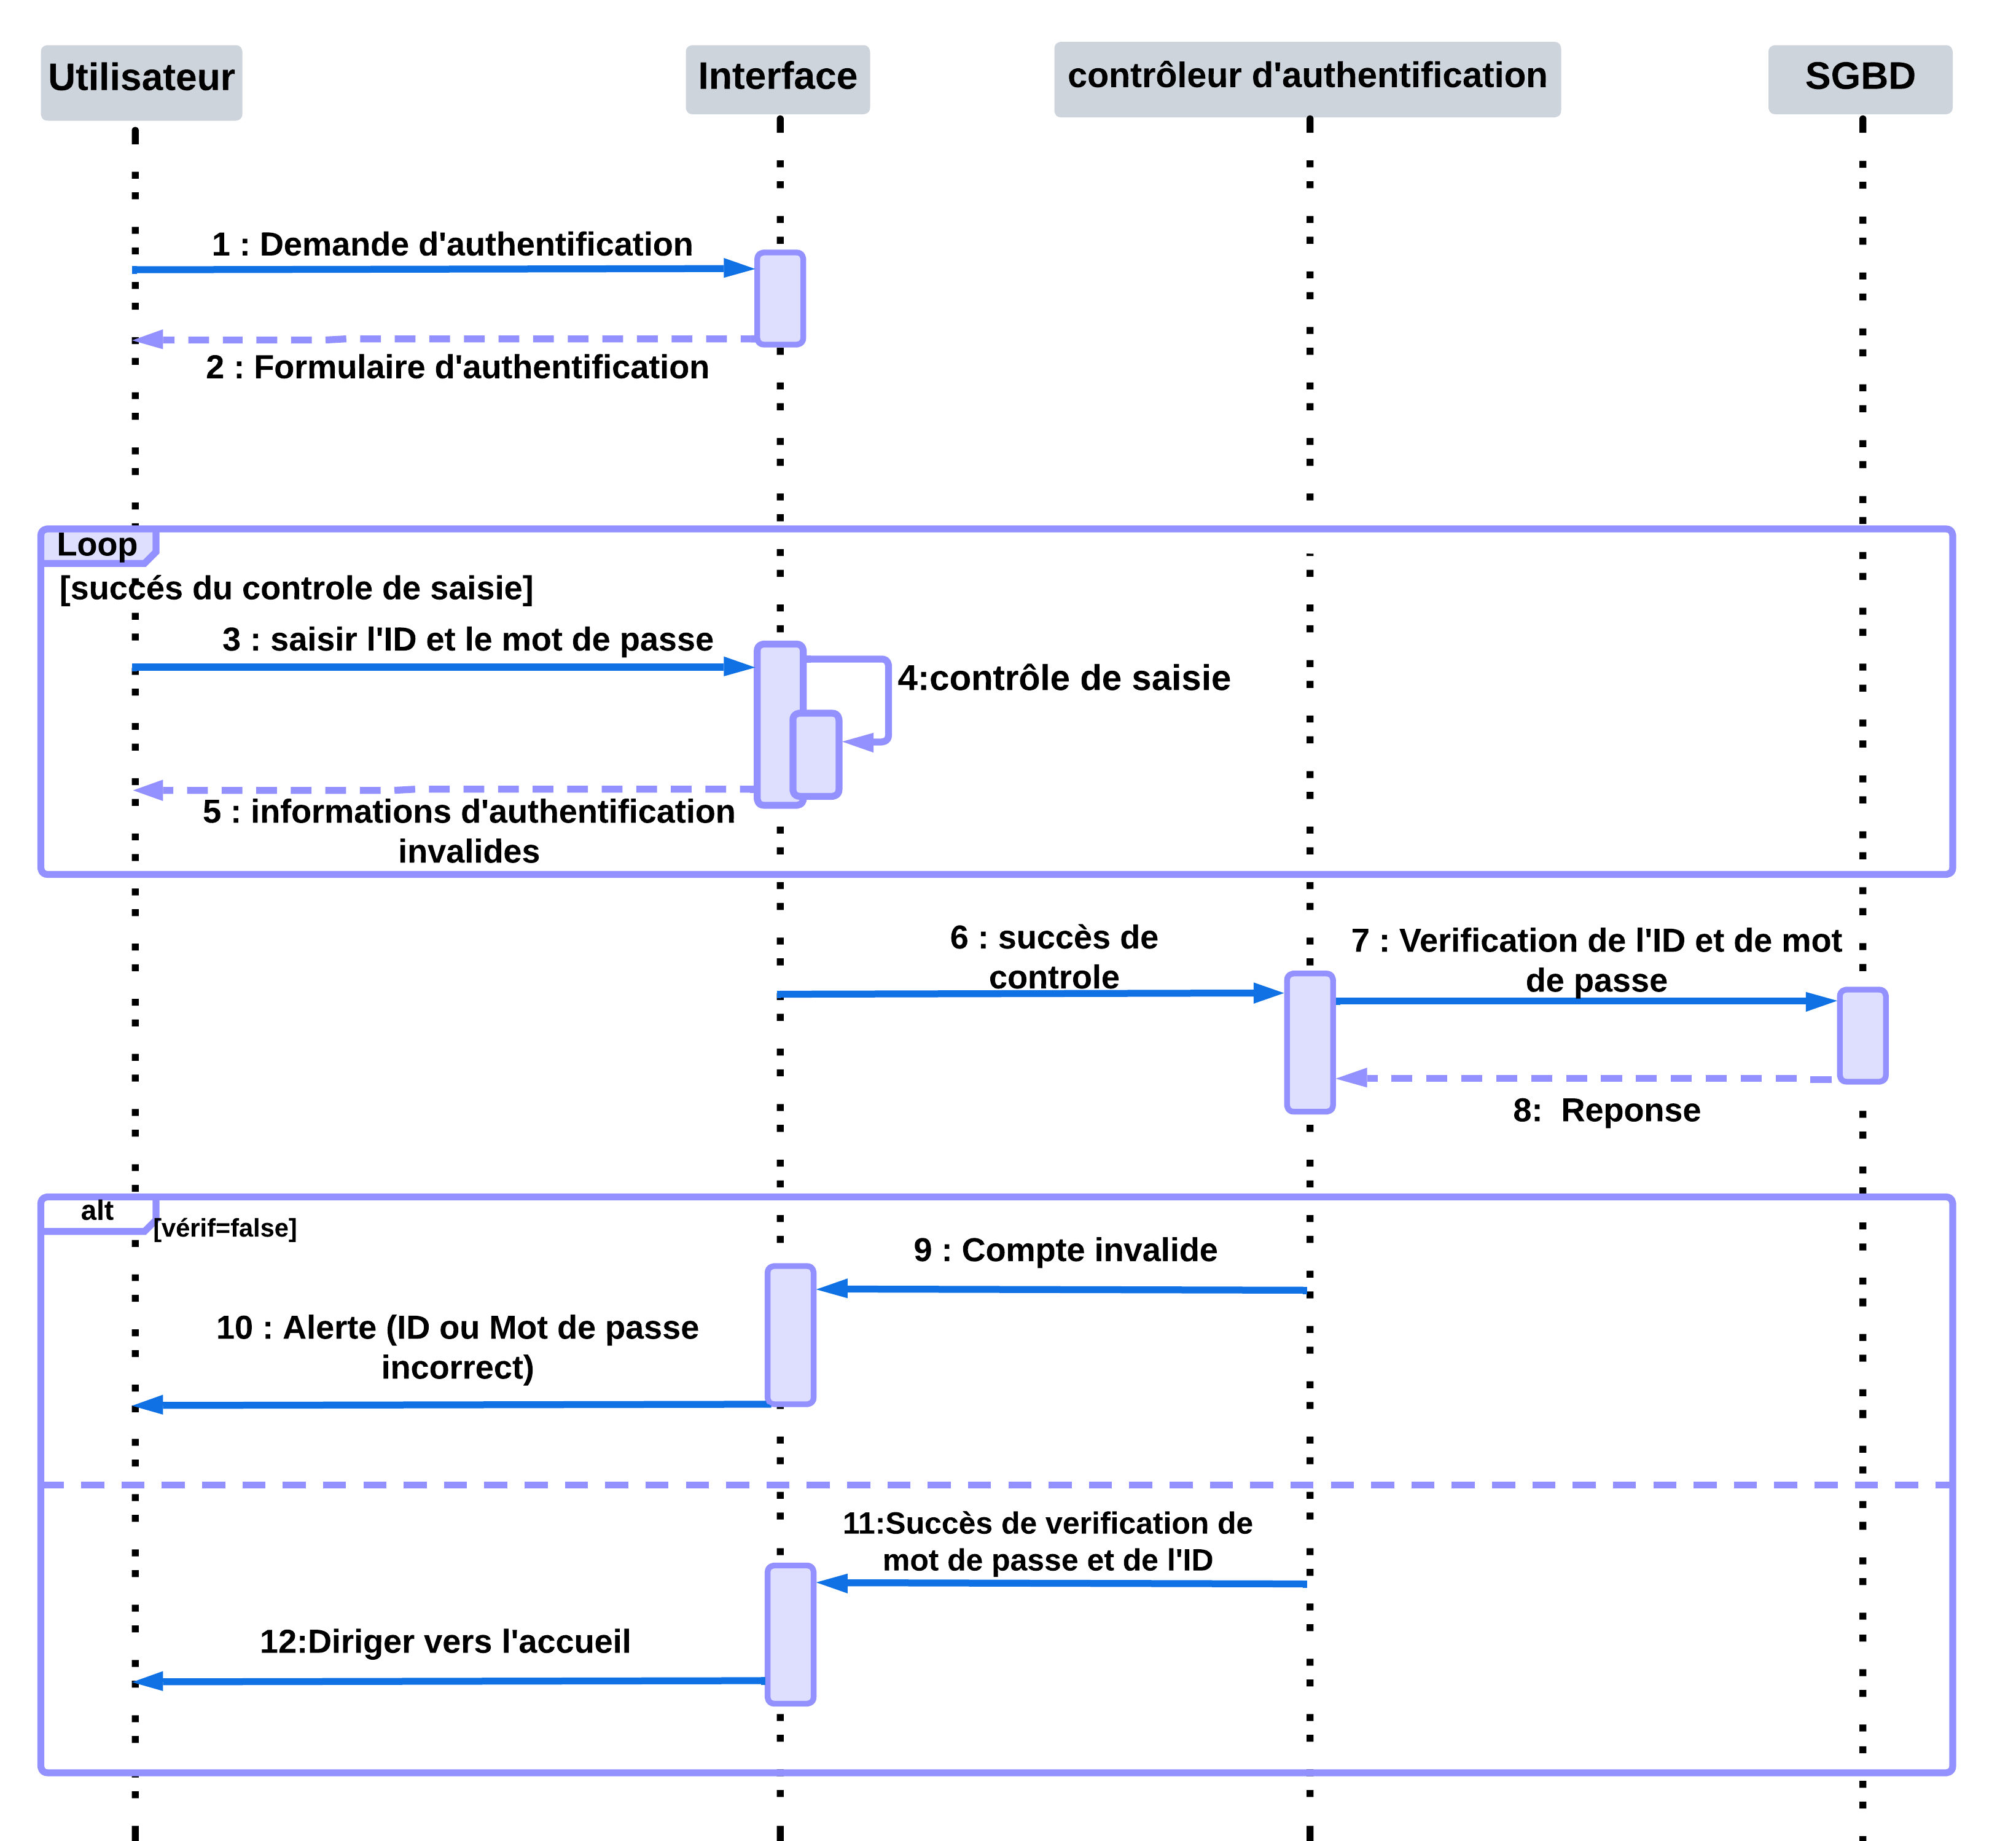
\includegraphics[width=18.5cm]{4}
  \caption{ Diagramme de séquence du cas d'utilisation << S'authentifier >>}
  \label{fig:votre-label}
\end{figure}
Pour s'authentifier, un administrateur/Employé doit saisir son identifiant et son mot de passe, si les données saisies sont correctes alors une session sera ouverte pour lui et il sera redirigé à la page d'accueil de l'application appropriée pour son espace. Si les données sont invalides alors un message d'erreur sera affiché demandant à l'utilisateur de saisir de nouveau l'identifiant et le mot de passe valides.
\subsubsection{Diagramme de séquence << Ajouter une facture >>}
\begin{figure}[H]
  \centering
  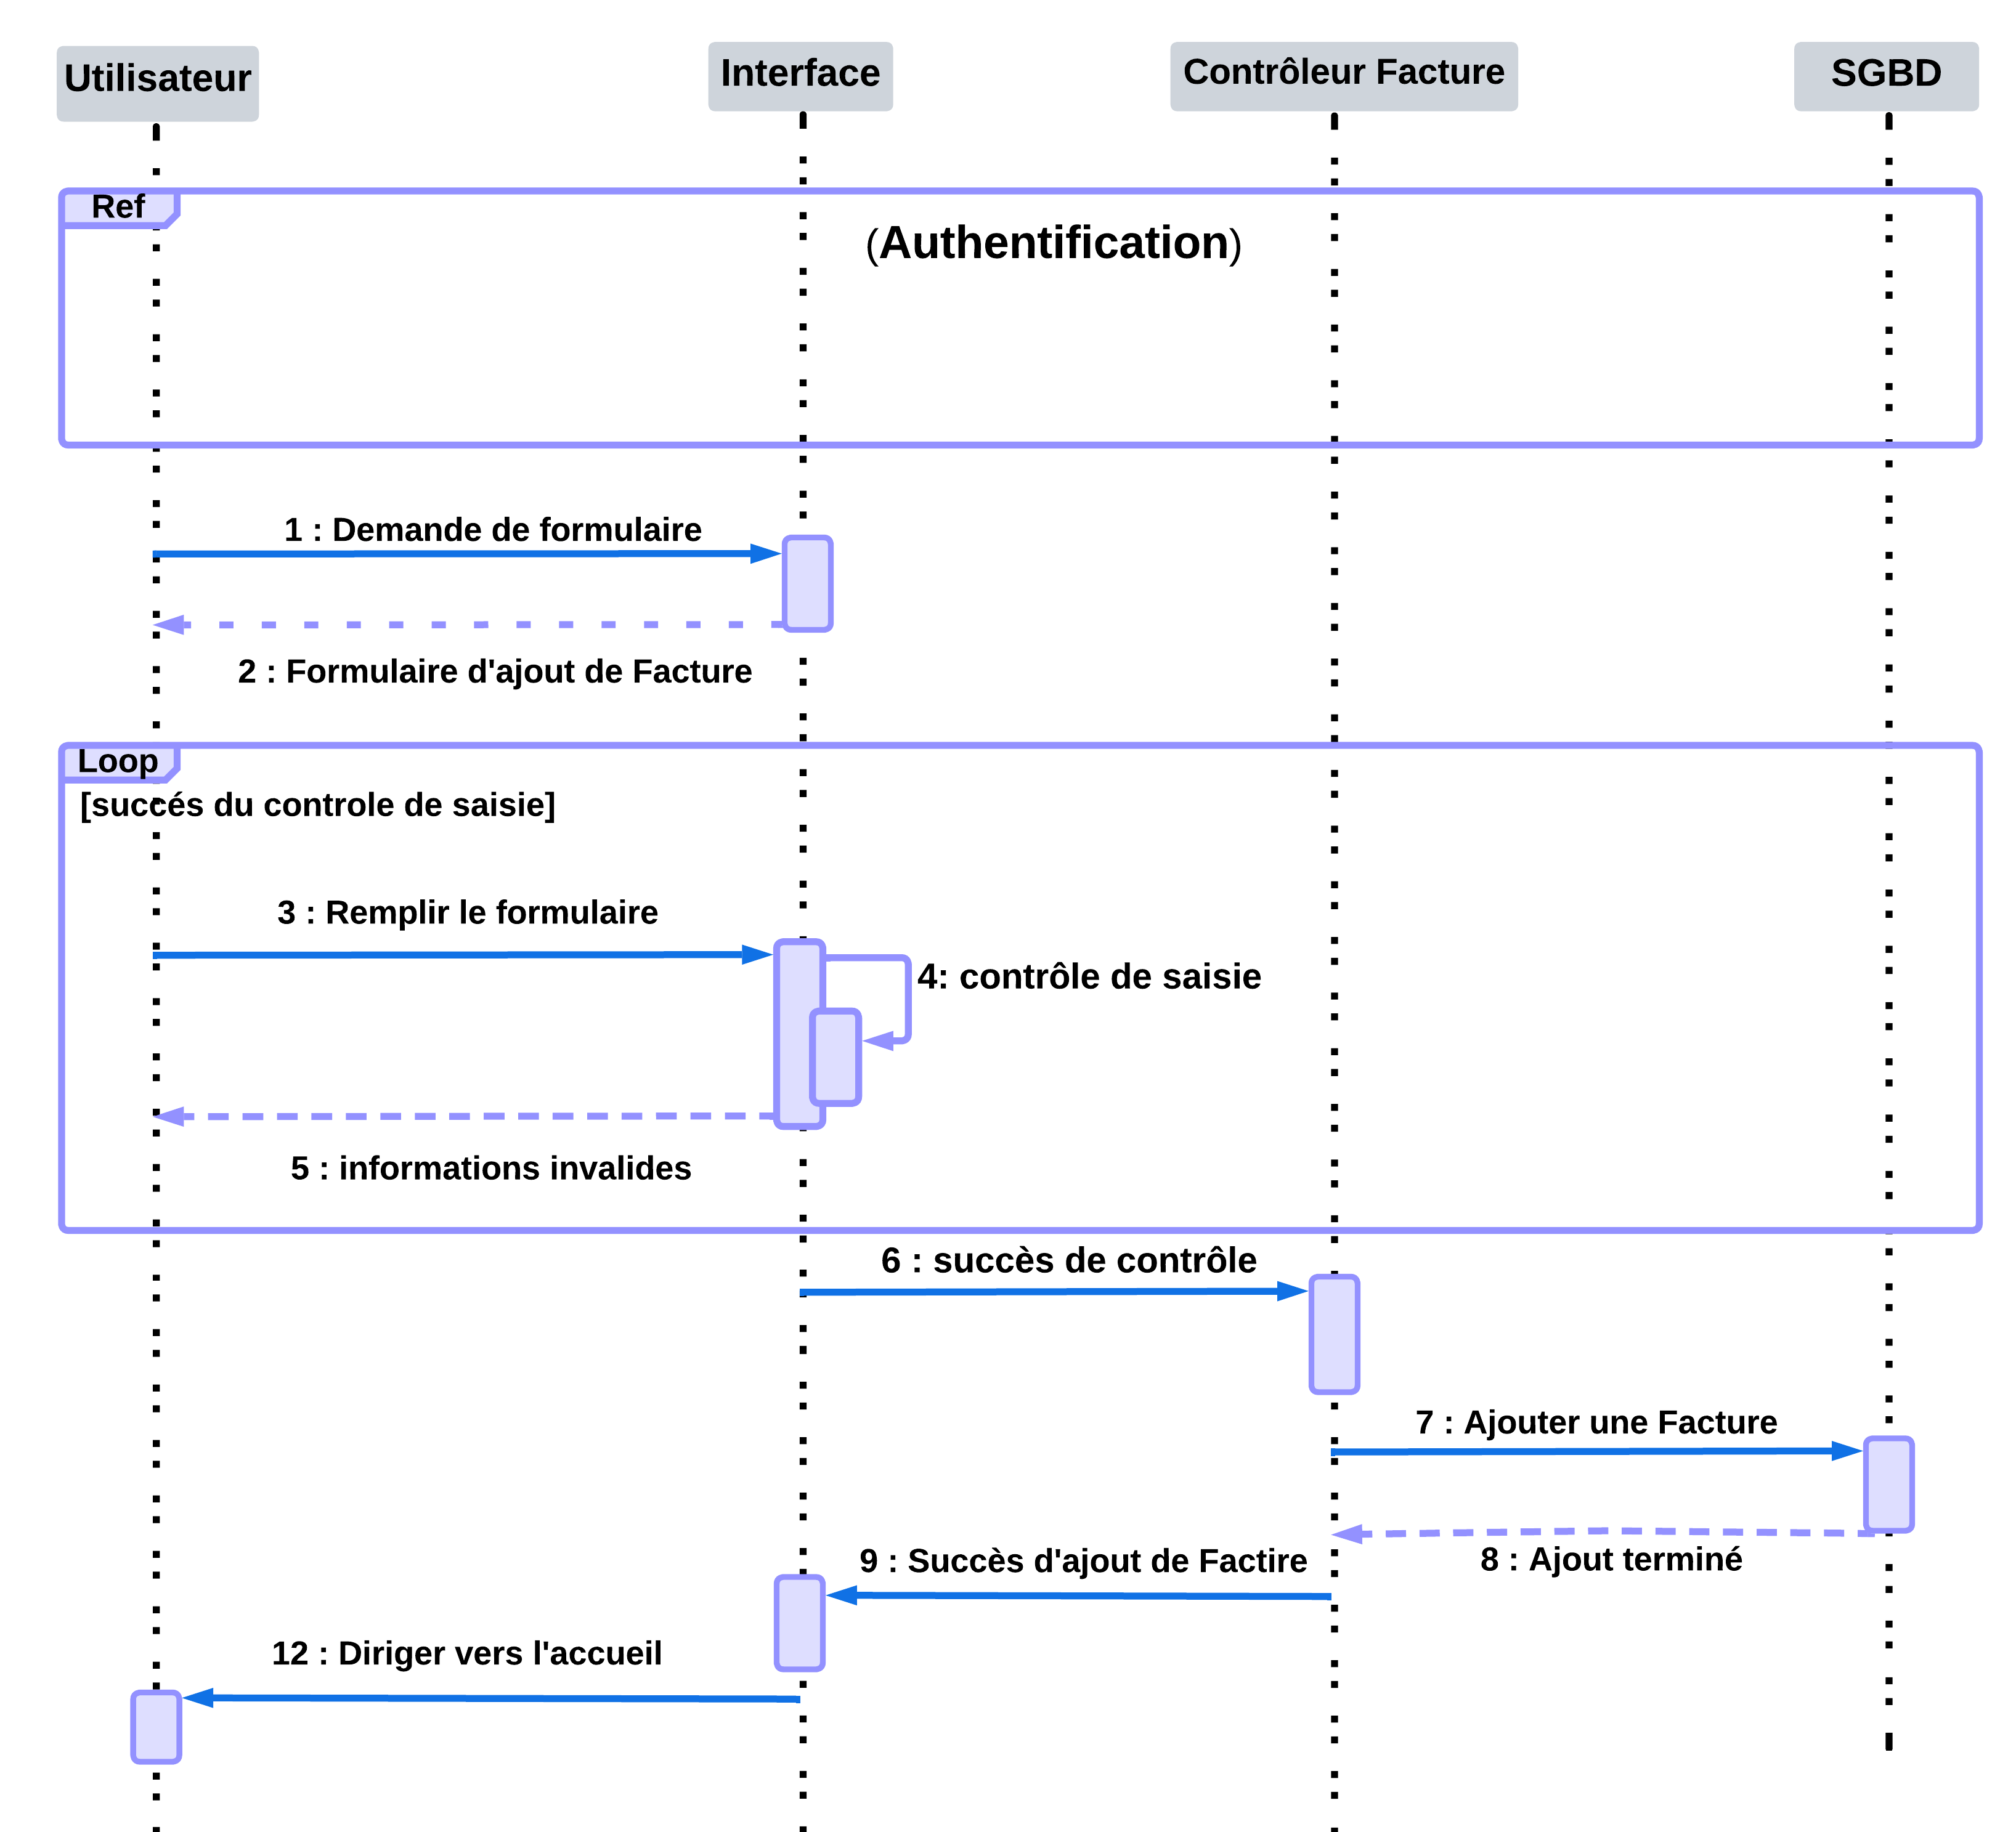
\includegraphics[width=18.5cm]{2}
  \caption{ Diagramme de séquence du cas d'utilisation << Ajouter une facture >>}
  \label{fig:votre-label}
\end{figure}
Pour Ajouter une facture, un administrateur/Employé doit être authentifié pour remplir le formulaire, si les informations saisies sont correctes alors la facture sera ajoutée avec succès . Si les informations sont erronées alors un message d'erreur seront affichées demandant à l'utilisateur de saisir de nouveau les données.
\section{Vue statique}
Le diagramme de cas d'utilisation décrit le système du point de vue acteurs.\\ Le diagramme de classe décrit la structure interne tout en présentant les différentes classes, leurs attributs, leurs méthodes ainsi que les différentes relations structurelles entre ces classes.\\ La figure 3.4 représente le diagramme de classes que nous avons utilisé pour développer notre application.
\begin{figure}[H]
  \centering
  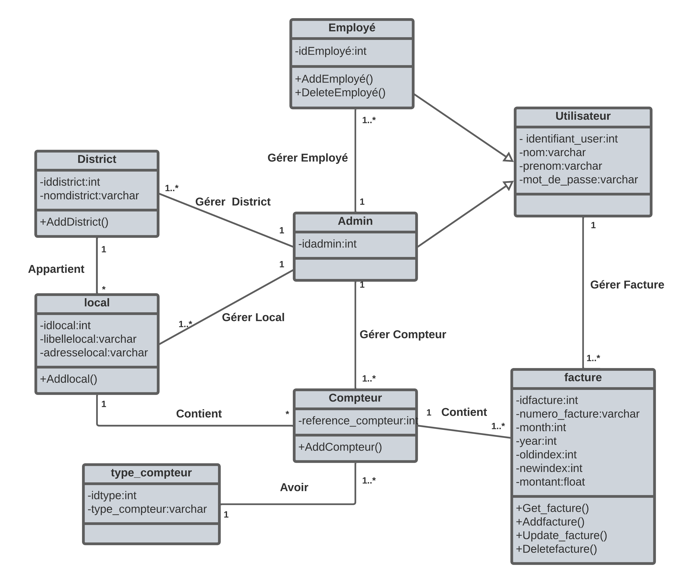
\includegraphics[width=19cm]{diagclasse2}
  \caption{ Diagramme de Classe}
  \label{fig:votre-label}
\end{figure}
\section*{Conclusion}
\addcontentsline{toc}{section}{Conclusion}

Durant ce chapitre, nous avons décrit l'architecture de notre système et nous avons présenté une vue statique à travers un diagramme de classes décrivant l'organisation du système et une vue dynamique à travers des diagrammes de séquences.
\\
Dans le chapitre suivant, nous allons passer à la réalisation de l'application.
%chapitre 4

\chapter{Réalisation de L'application}
\vspace{100pt}
\begin{center}
Plan du chapitre
\end{center}

\hrule
\vspace{20pt}
Introduction
\begin{enumerate}
	\item Environnements du travail
	\item Interfaces graphiques de l'application
	\item chronogramme de réalisation
\end{enumerate}

Conclusion
\vspace{20pt}
\hrule

\newpage
\section*{Introduction}
\addcontentsline{toc}{section}{Introduction}
Après avoir effectué l'étude et la conception de L'application, ce chapitre concerne la phase de réalisation. En d'autres termes, cette dernière section est dédiée aux résultats obtenus par notre application.\\ À cette fin, nous présenterons d'abord l'environnement matériel et logiciel supportant notre Site. Après cela, nous présentons la plateforme de développement et les choix technologiques.
\subsection{Environnements du travail}
Tout au long de la réalisation de notre application, nous avons utilisé des matériels et des logiciels.
\subsubsection{Environnements de développement matériel}
Pour la réalisation du projet, nous avons utilisé un Ordinateur portable Lenovo pour le développement:
\vspace{0.2cm}
\begin{table}[H]
\centering
\def\arraystretch{2.5}
\begin{tabular}{||p{5cm}||p{10cm}||}
   \hline
   \hline
   \begin{large}
    \textbf{Système d'exploitation}
   \end{large} & Windows 10\\
   \hline
   \hline
   \begin{large}
    \textbf{disque dur}
   \end{large} & 1 To \\
   \hline
   \hline
   \begin{large}
    \textbf{Ram}
   \end{large} & 8 Go\\
   \hline
   \hline
   \begin{large}
    \textbf{Processeur}
   \end{large} & Intel(R) Core(TM) i3-8145U CPU @ 2.10GHz   2.30 GHz\\
   \hline
   \hline
\end{tabular}
\caption{caractéristiques de l'ordinateur}
\end{table}
\vspace{0.5cm}
\subsubsection{Environnements de développement logiciel}
Dans cette partie,nous nous concentrons aux langages ,aux bibliothèques et aux techniques de programmation utilisées pendant le développement de notre application.
\newpage
\textbf{A. IDE de développement :}

\begin{table}[H]

\def\arraystretch{1}
\begin{tabular}{||p{5cm}||p{12cm}||}
   \hline
   \hline
   \vspace{0.8cm}
   \centering
   
\includegraphics[width=0.13\textwidth, height=20mm]{visual.png}\\
   \vspace{1cm}
   
   &
   \vspace{0.5cm}
   \begin{doublespace}
    \textbf{Visual Studio Code:} est un éditeur de code extensible dévloppé 
par Microsoft pour Windows, Linux et macOS. Il est multiplateforme, open source et gratuit, supportant une dizaine de langages.\end{doublespace}
   \\
   \hline
   \hline  
\end{tabular} 
\end{table}
\textbf{B. SGBD :} 
\begin{table}[H]
\def\arraystretch{2}
\begin{tabular}{||p{5cm}||p{12cm}||} 
	\hline
	\hline
   \vspace{1.5cm}
   \centering
   
\includegraphics[width=0.2\textwidth, height=15mm]{mysql.png}\\
   \vspace{1cm}
   &
   
   \begin{doublespace}
    \textbf{MySQL :} est un système de gestion de bases de données relationnelles utilisant le langage de programmation SQL. Il propose une version open source qui permet à l'utilisateur d'accéder au code source et de le modifier, et une version entreprise permettant un accès aux dernières fonctionnalités du logiciel et au support fourni par Oracle, propriétaire et développeur actuel de MySQL \end{doublespace}
   \\ 
   \hline
   \hline
\end{tabular}   
\end{table}

\textbf{C. Langage de programmation :}
\begin{table}[H]
\def\arraystretch{0.5}
\begin{tabular}{||p{5cm}||p{12cm}||} 
   \hline
   \hline
   \vspace{1.5cm}
   \centering
   
\includegraphics[width=0.15\textwidth, height=20mm]{python.png}\\
   \vspace{0.5cm}
   &
   \begin{doublespace}
   \vspace{1cm}
    \textbf{Python :} est un langage de programmation de haut niveau, interprété et polyvalent, largement utilisé dans le développement logiciel, la science des données, l'automatisation de tâches, la création de sites web et bien d'autres domaines\end{doublespace}
   \\
   \hline
   \hline
  
\end{tabular}

\end{table}

\textbf{D. Bibliothèque :}
Dans le cadre de ce projet, j'ai choisi de développer l'interface graphique de mon application bureau à l'aide de la bibliothèque Tkinter.
\begin{table}[H]

\def\arraystretch{0.8}
\begin{tabular}{||p{17cm}||}    
   \hline
   \hline
   \vspace{0.2cm}
 
   \begin{doublespace}
    \textbf{Tkinter :} est un module embarqué en Python qui fournit des outils puissants pour créer des interfaces utilisateur conviviales. Tkinter est une bibliothèque bien documentée et largement utilisée pour créer des interfaces graphiques, ce qui la rend idéale pour le développement de mon application.

L'un des principaux avantages de Tkinter est sa flexibilité dans la personnalisation de l'interface. J'ai pu créer des fenêtres, des boutons, des zones de texte et d'autres contrôles en quelques lignes de code Python. Cette flexibilité m'a permis de conserver une interface claire et conviviale tout en répondant aux besoins spécifiques de mon application. Tkinter propose également une grande variété d'interactions telles que des boîtes de dialogue, des barres de progression et des événements de clic de souris pour améliorer l'expérience utilisateur. \end{doublespace}
   \\
   \hline
   \hline
\end{tabular}
\end{table}

\section{Interfaces graphiques de l'application}
Les Figuresci-dessous représentent les différentes interfaces de l'application :

\subsection{Interface d'authentification:}

\begin{figure}[H]
  \centering
  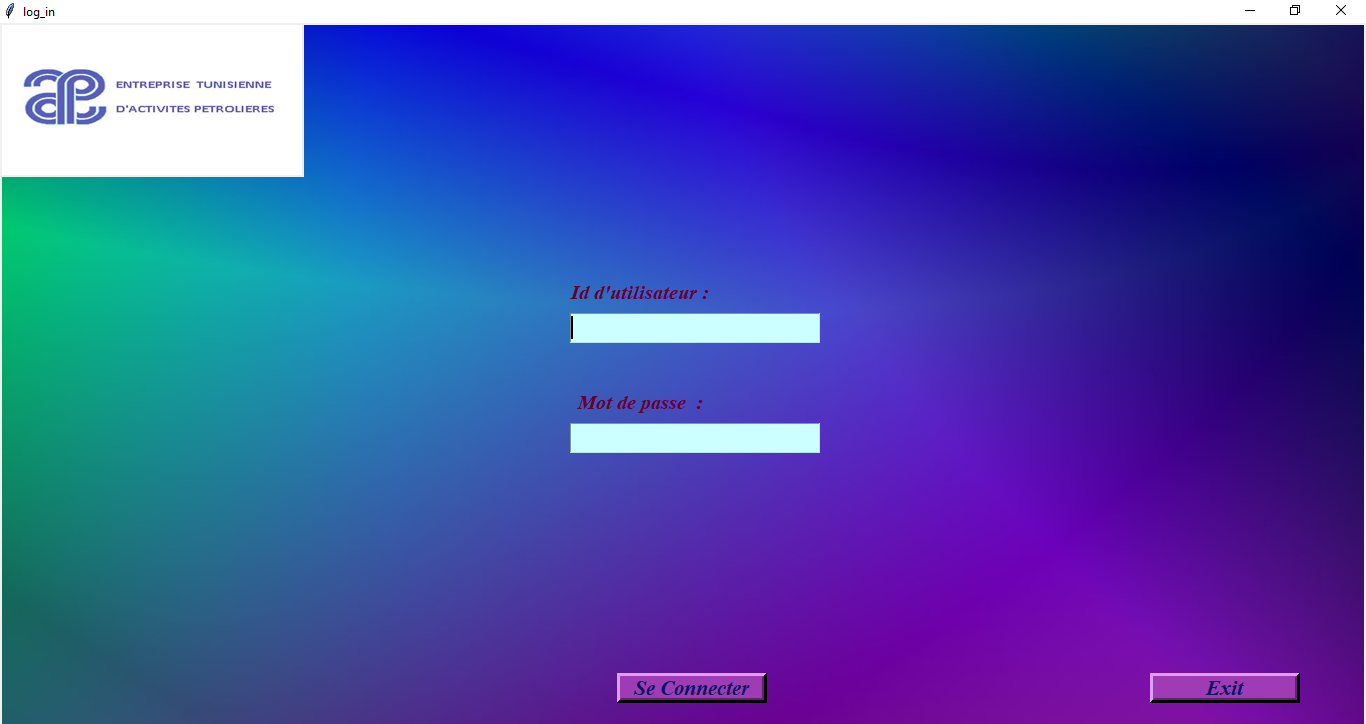
\includegraphics[scale=0.47]{login}
  \caption{Interface : Authentification}
  \label{fig:votre-label}
\end{figure}
\newpage
\subsection{L'interface d'accueil }
L'employé peut ajouter des factures et il est seulement autorisé à consulter les factures qu'il a ajoutées.
\begin{figure}[H]
  \centering
  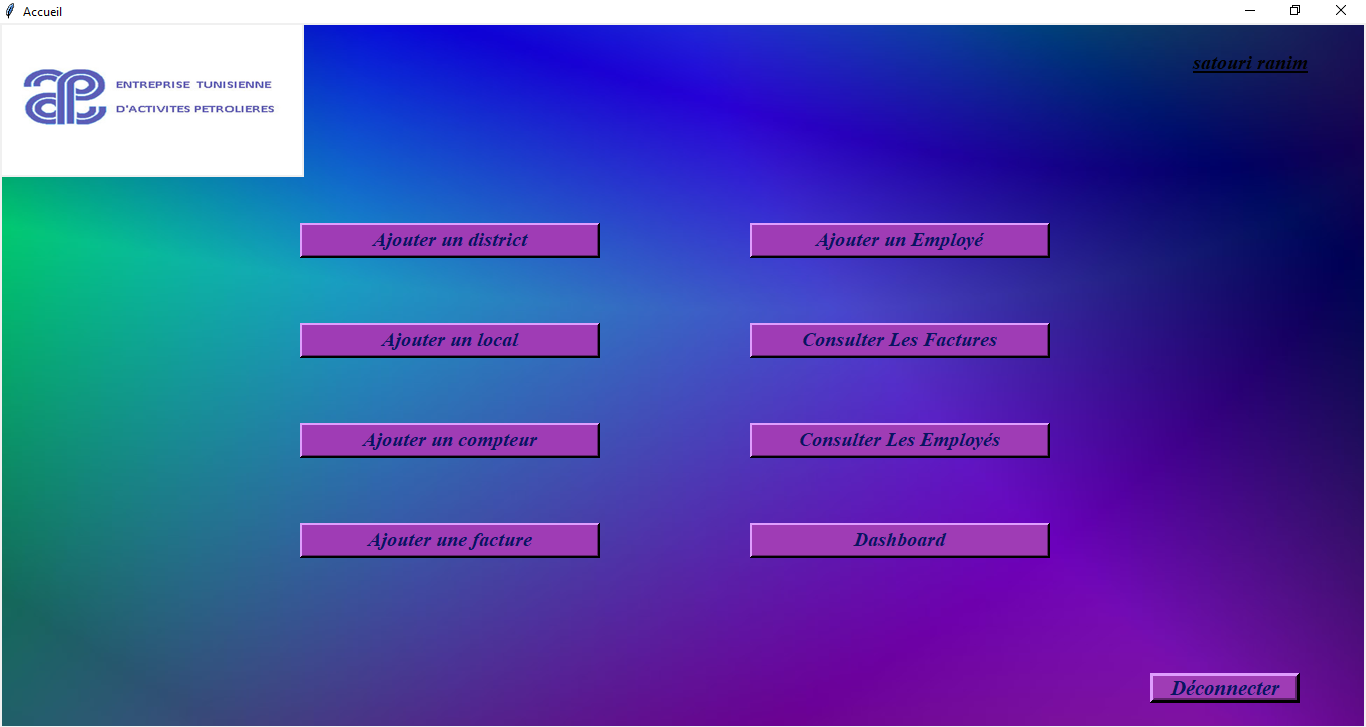
\includegraphics[scale=0.47]{accueil}
  \caption{Interface : Accueil de l'administrateur}
  \label{fig:votre-label}
\end{figure}
\begin{figure}[H]
  \centering
  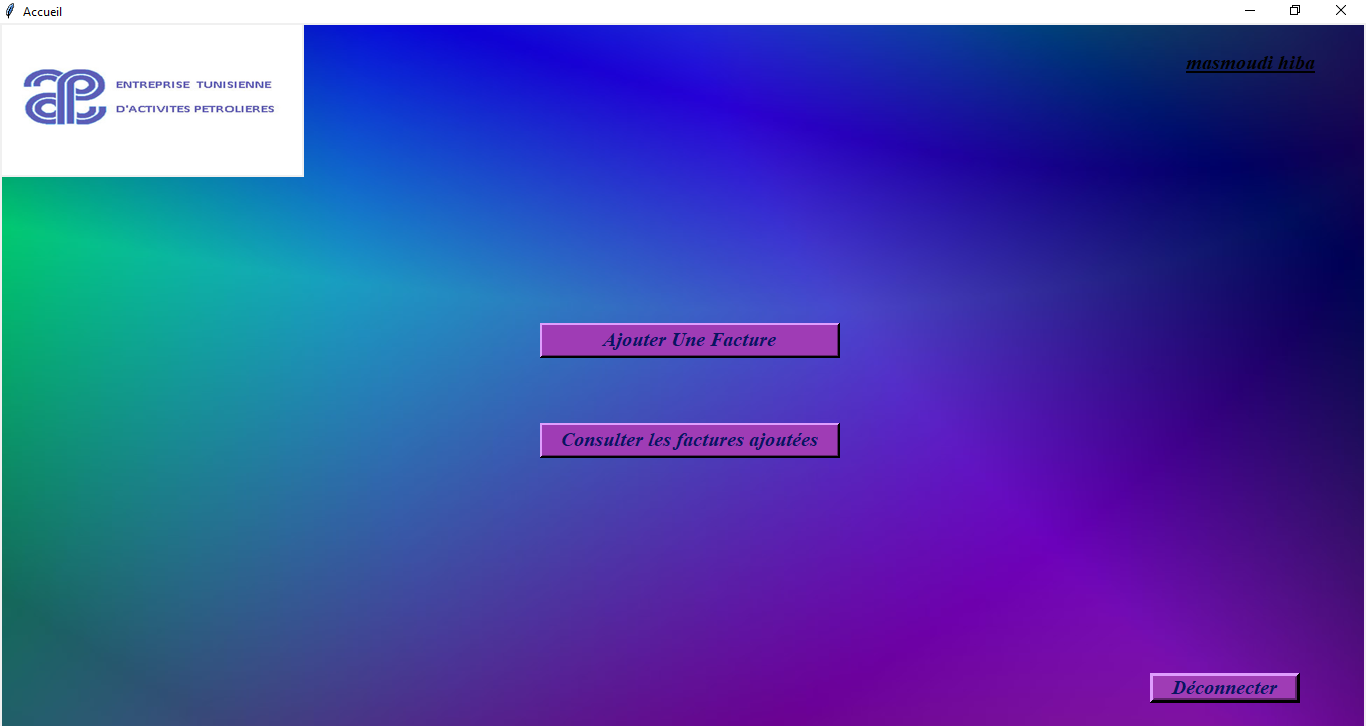
\includegraphics[scale=0.47]{acceuil_user}
  \caption{Interface : Accueil de l'Employé}
  \label{fig:votre-label}
\end{figure}
\subsection{Les interfaces d'ajout }
\begin{figure}[H]
  \centering
  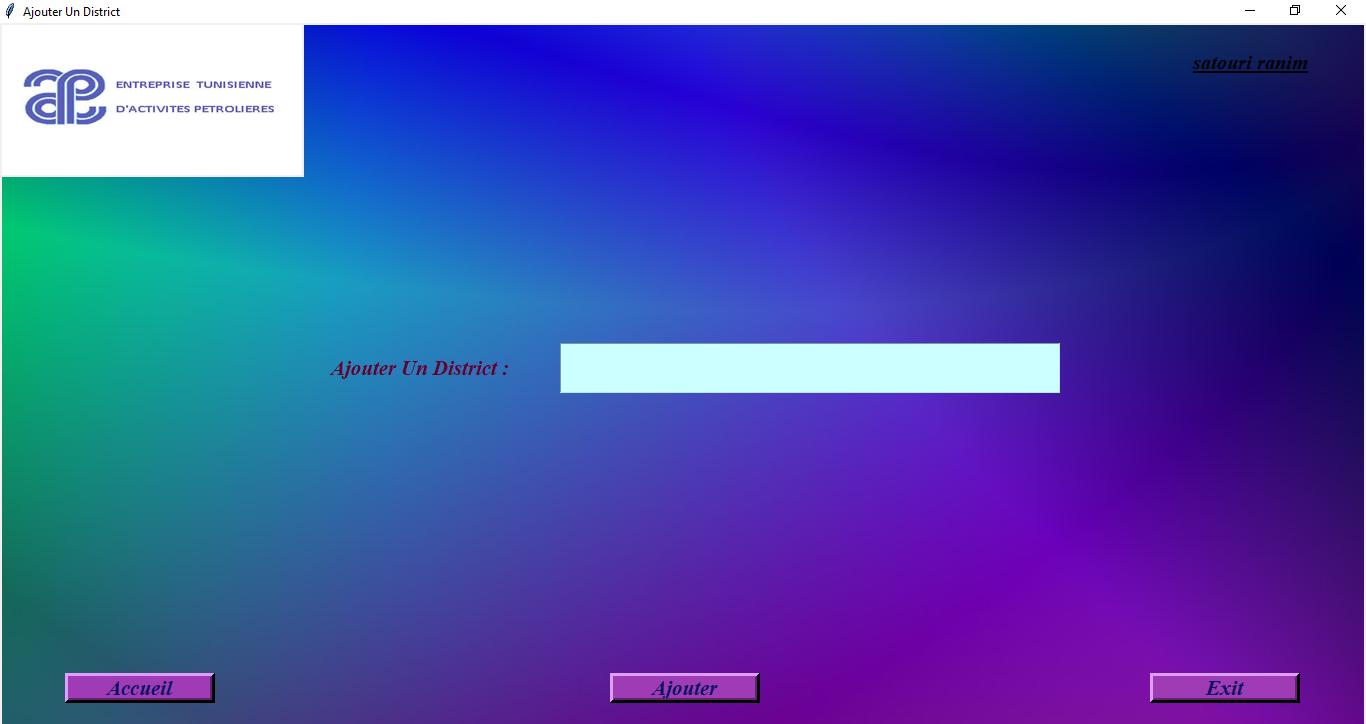
\includegraphics[scale=0.47]{add_district}
  \caption{Interface : Ajouter un district}
  \label{fig:votre-label}
\end{figure}
\begin{figure}[H]
  \centering
  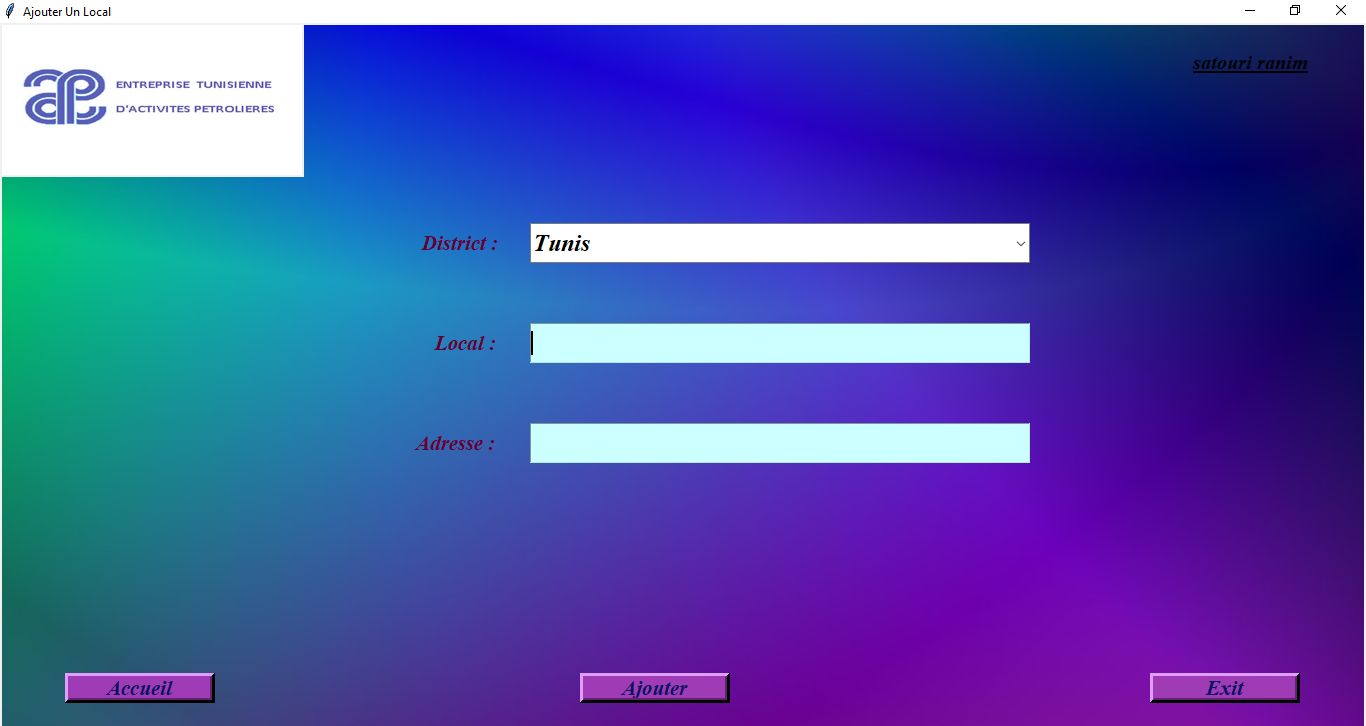
\includegraphics[scale=0.47]{add_local}
  \caption{Interface : Ajouter un Local}
  \label{fig:votre-label}
\end{figure}
\begin{figure}[H]
  \centering
  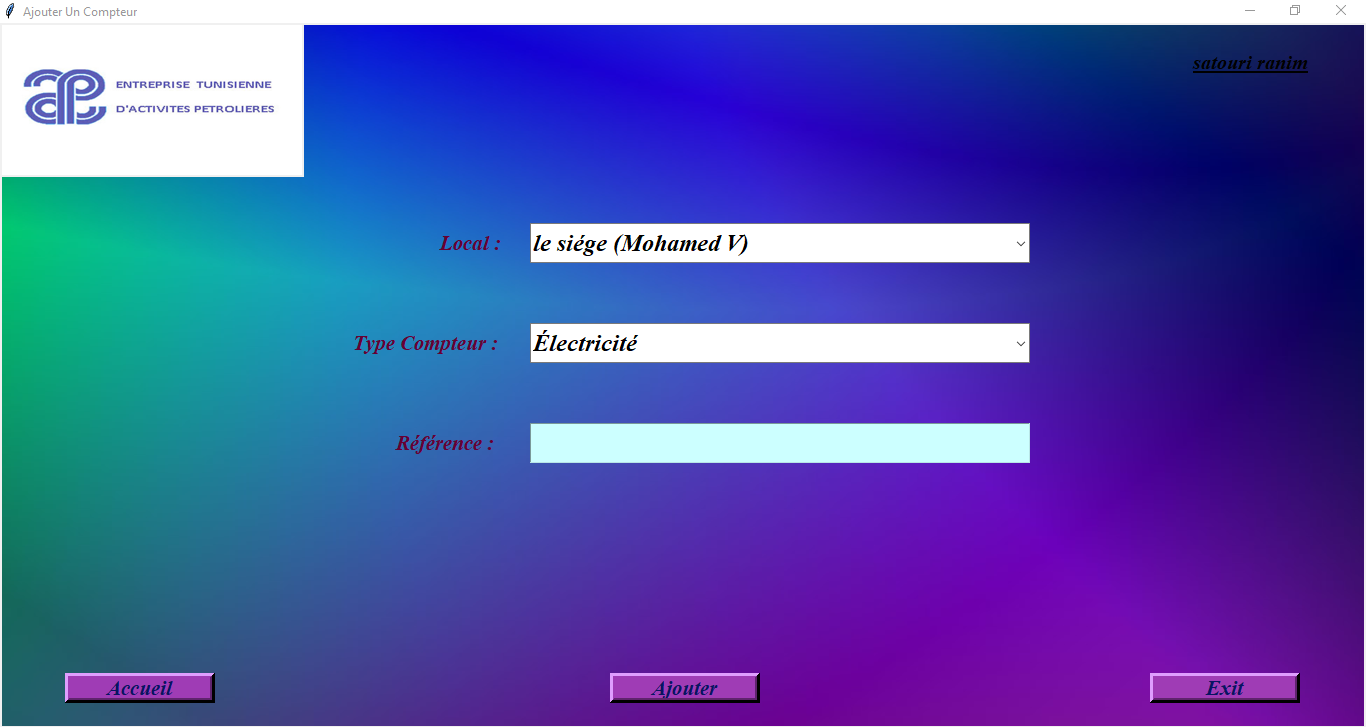
\includegraphics[scale=0.47]{add_compteur}
  \caption{Interface : Ajouter un compteur}
  \label{fig:votre-label}
\end{figure}
\begin{figure}[H]
  \centering
  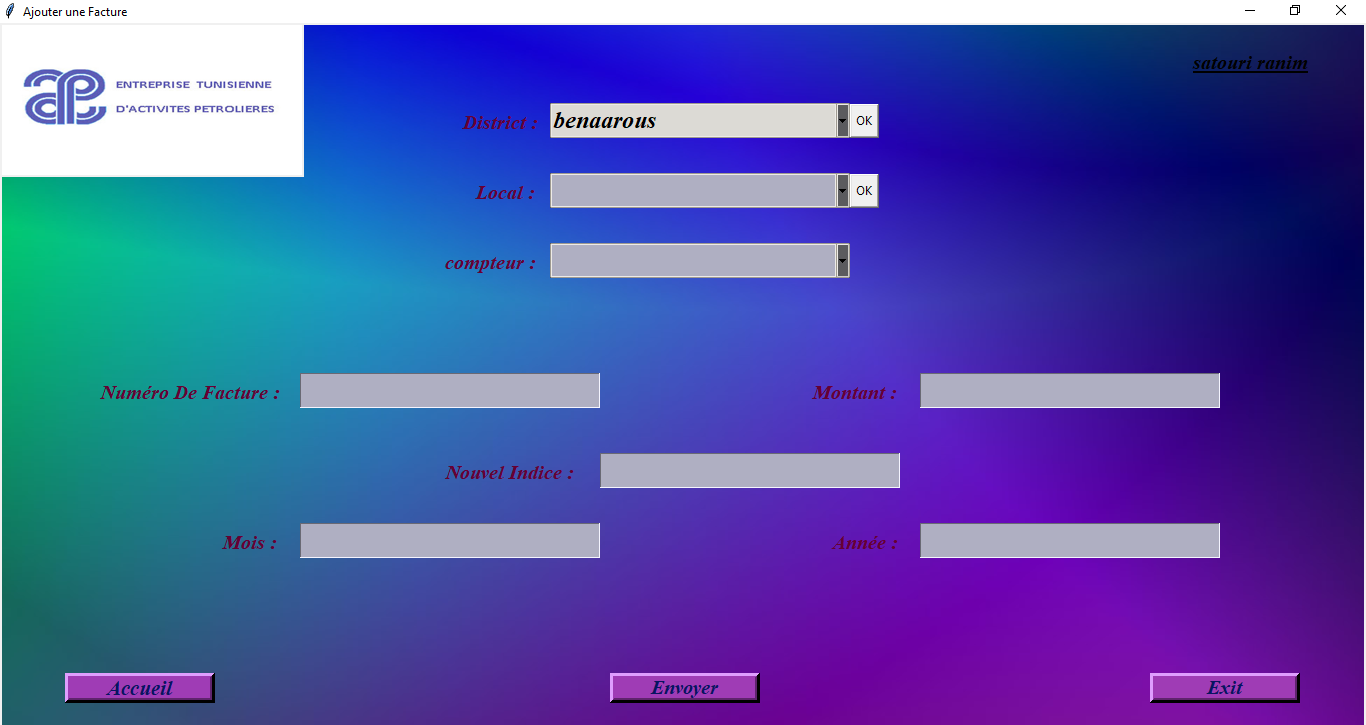
\includegraphics[scale=0.47]{add_facture}
  \caption{Interface : Ajouter une facture}
  \label{fig:votre-label}
\end{figure}
\begin{figure}[H]
  \centering
  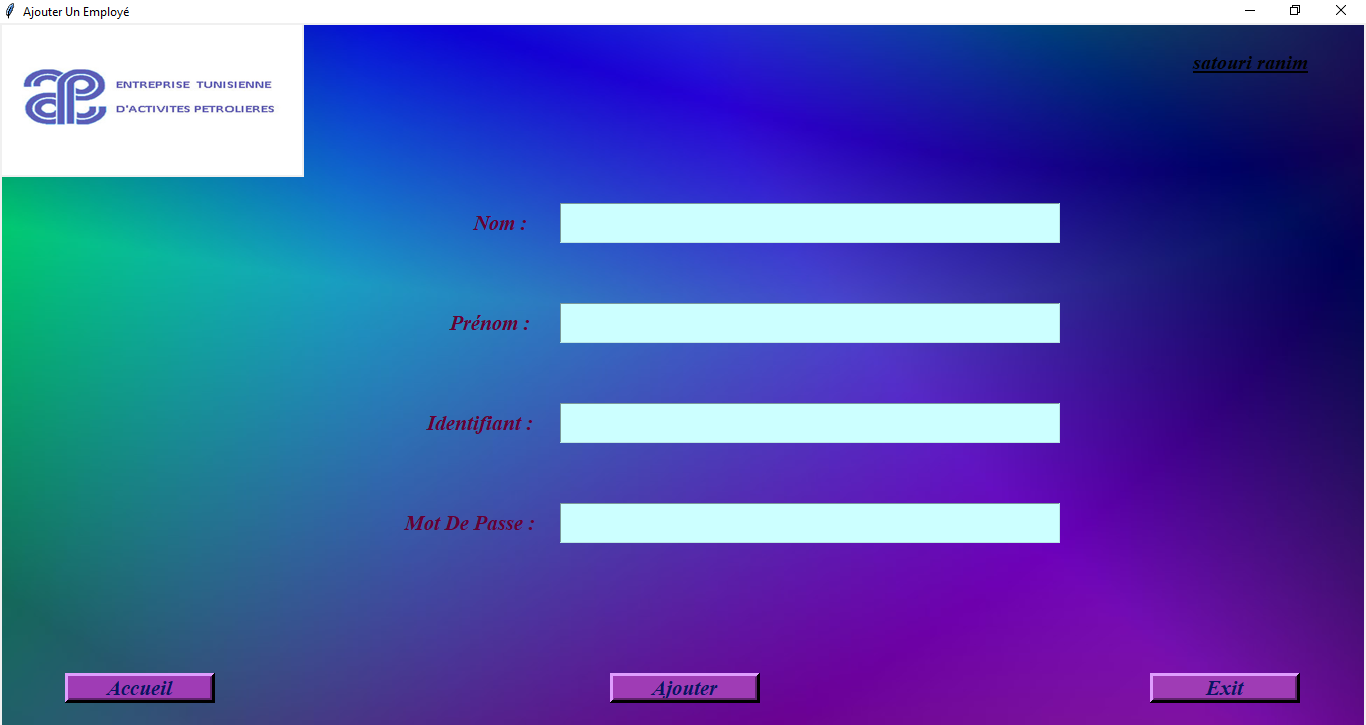
\includegraphics[scale=0.47]{add_user}
  \caption{Interface : Ajouter un Employé}
  \label{fig:votre-label}
\end{figure}
\subsection{interface Admin pour gérer les Factures}
\begin{figure}[H]
  \centering
  \includegraphics[scale=0.47]{Get_facture}
  \caption{Interface : Consulter les Factures}
  \label{fig:votre-label}
\end{figure}
\begin{figure}[H]
  \centering
  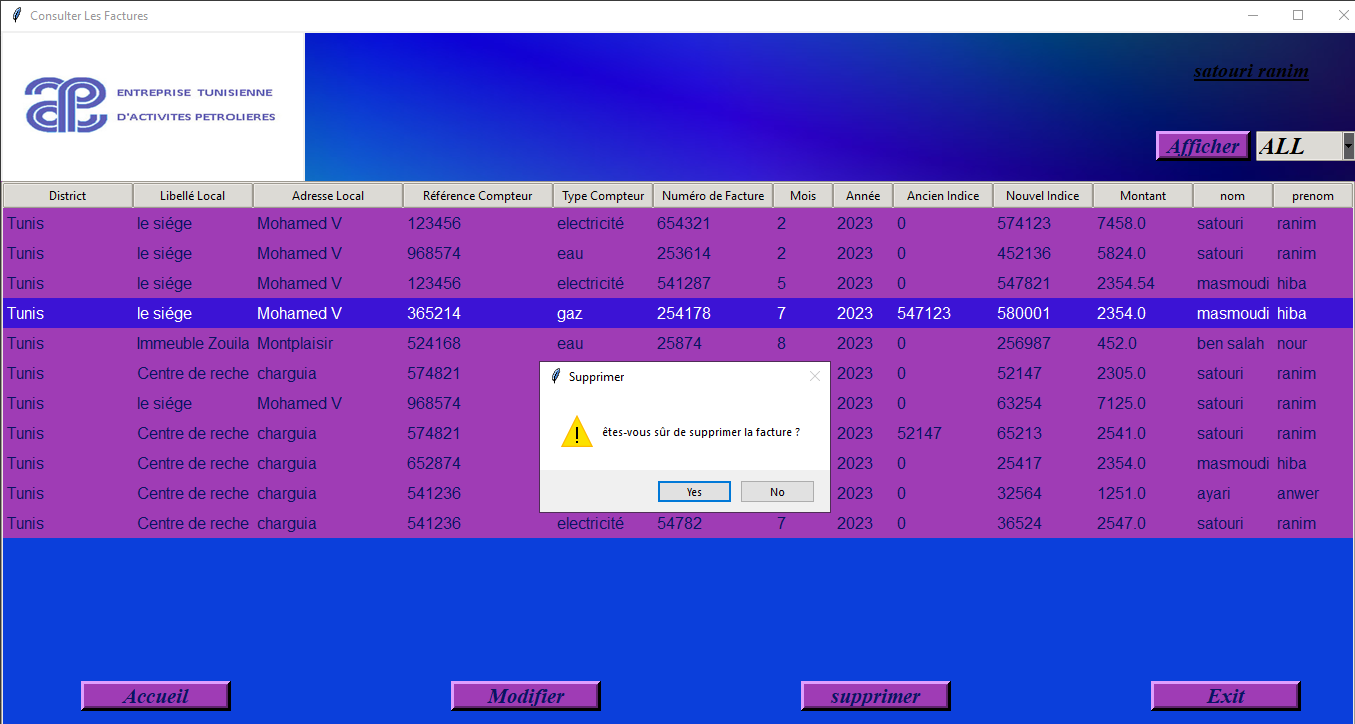
\includegraphics[scale=0.47]{delete_fact}
  \caption{Interface : Confirmer la suprission d'une facture}
  \label{fig:votre-label}
\end{figure}
\begin{figure}[H]
  \centering
  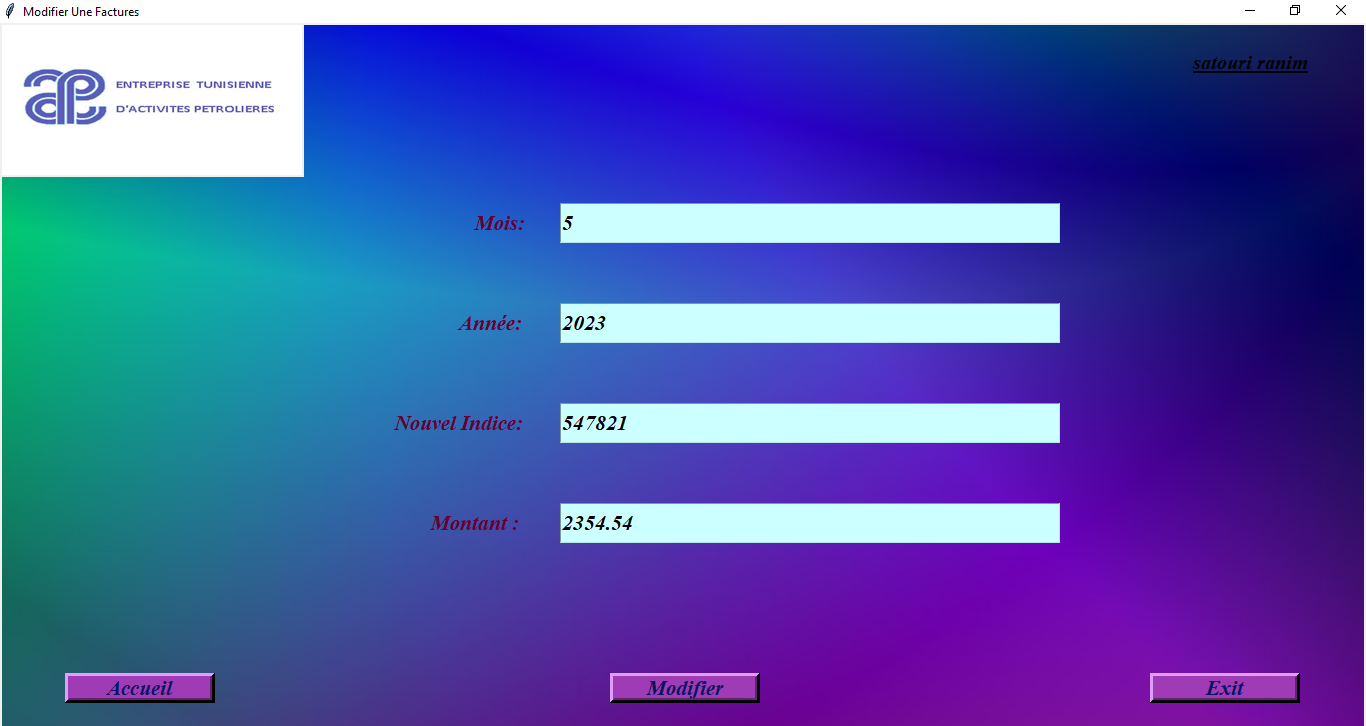
\includegraphics[scale=0.47]{update_fact}
  \caption{Interface : Modifier une facture}
  \label{fig:votre-label}
\end{figure}
\subsection{Interface admin pour gérer les Employés}
\begin{figure}[H]
  \centering
  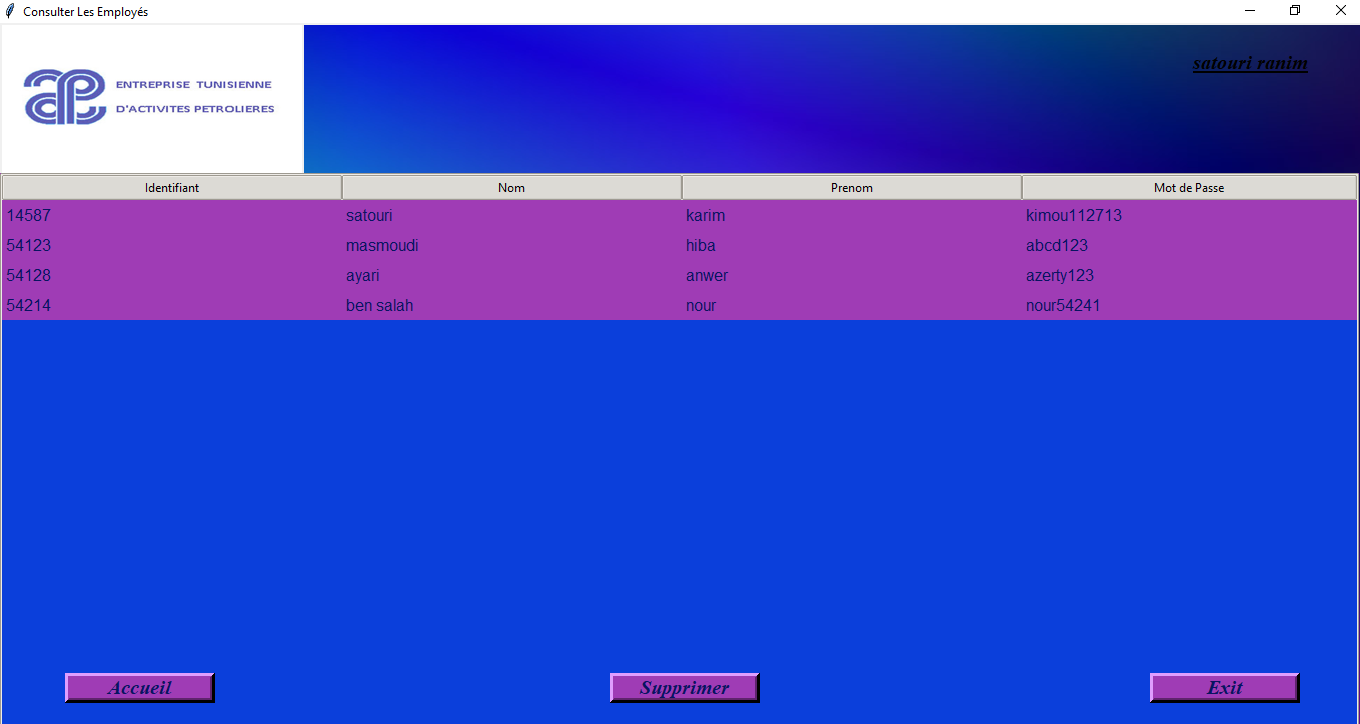
\includegraphics[scale=0.47]{get_user}
  \caption{Interface : consulter les Employés}
  \label{fig:votre-label}
\end{figure}
\subsection{Interface d'états statistiques }
\begin{figure}[H]
  \centering
  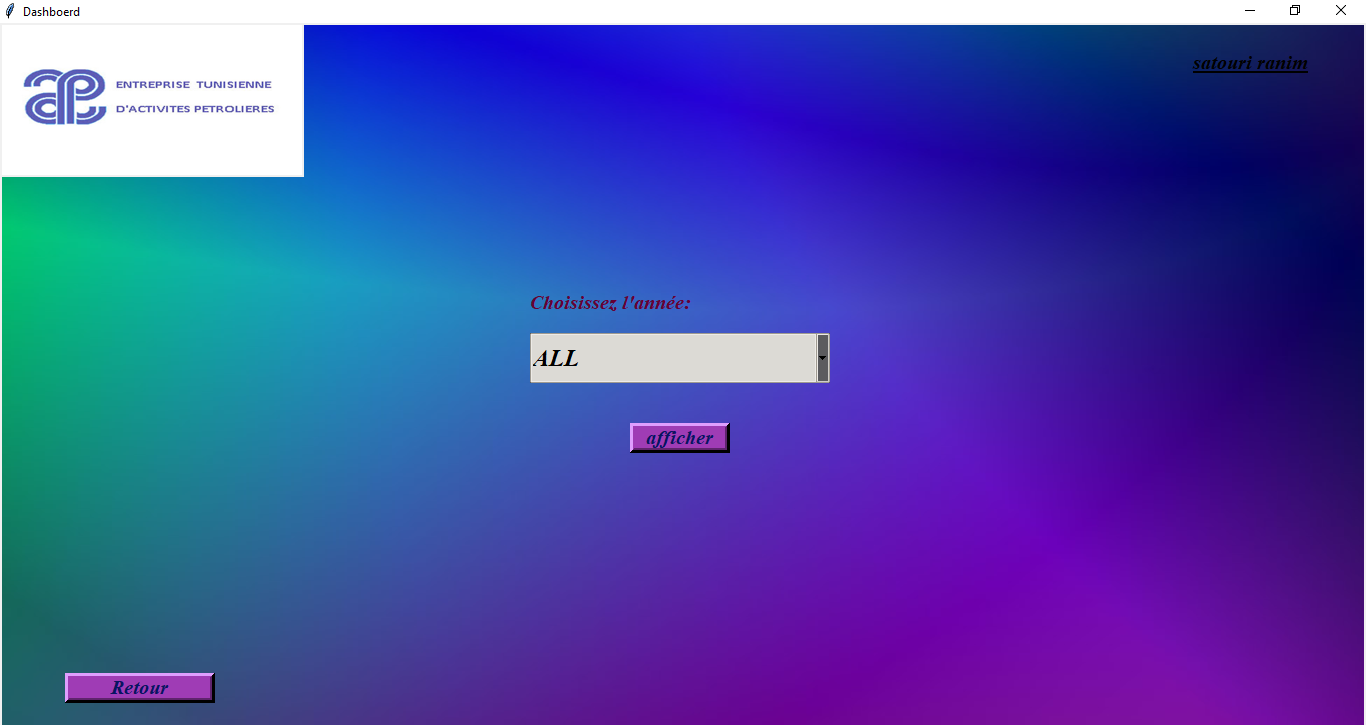
\includegraphics[scale=0.47]{dash1}
  \caption{Interface : selectionner l'année}
  \label{fig:votre-label}
\end{figure}
\begin{figure}[H]
  \centering
  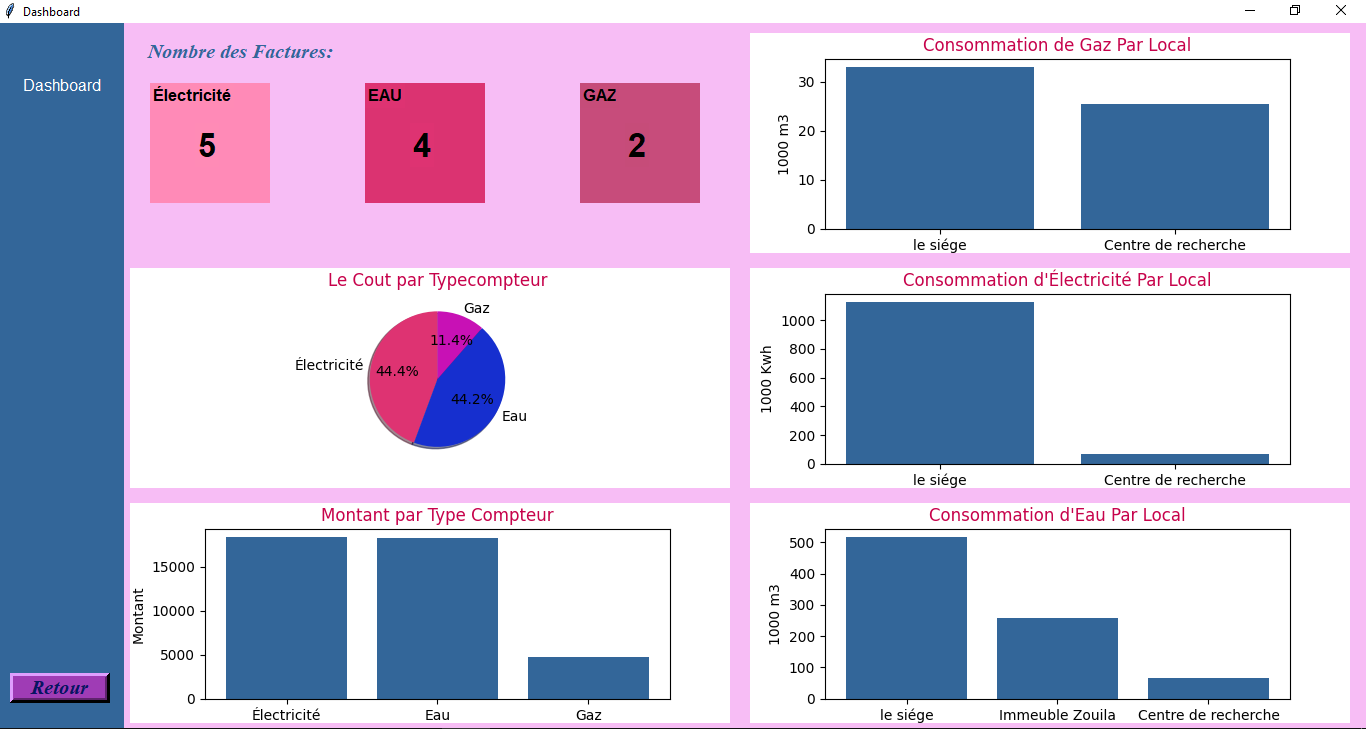
\includegraphics[scale=0.47]{dash2}
  \caption{Interface : dashboard}
  \label{fig:votre-label}
\end{figure}
\section{Chronogramme de réalisation du projet}
Le diagramme de Gantt est un outil utilisé en gestion de projet et permettant de visualiser dans le temps les diverses tâches composant un projet. Il permet de représenter graphiquement l'avancement de ce dernier.
Pour le bon déroulement de notre projet, la figure présente notre diagramme de Gantt, schématisé en respectant le planning de réalisation de nos tâches tout au long de la période de notre stage, présenté dans le tableau 4.2.
\begin{table}[H]
\centering
\def\arraystretch{2}
\begin{tabular}{|p{5cm}|p{3.5cm}|p{3.5cm}|p{3.5cm}|}
   \hline
   \begin{large}
    \textbf{Nom de tache}
   \end{large} &  
   \begin{large}
    \textbf{Durée}
   \end{large}
   &
   \begin{large}
    \textbf{Début}
   \end{large}
   &
   \begin{large}
    \textbf{Fin}
   \end{large}\\
   \hline
   \begin{large}
    \textbf{Spécification des besoins}
   \end{large} & 3 jours & 01/08/2023 & 03/08/2023\\
   \hline
   \begin{large}
    \textbf{Conception}
   \end{large} & 5 jours & 04/08/2023 & 08/08/2023 \\
   \hline
   \begin{large}
    \textbf{Développement}
   \end{large} & 23 jours & 09/08/2023 & 31/08/2023\\
   \hline
   \begin{large}
    \textbf{Rapport}
   \end{large} & 10 jours & 22/08/2023 & 31/08/2023\\
   \hline
\end{tabular}
\caption{Planning de réalisation des tâches tout au long de la période de stage}
\end{table}
\begin{figure}[H]
  \centering
  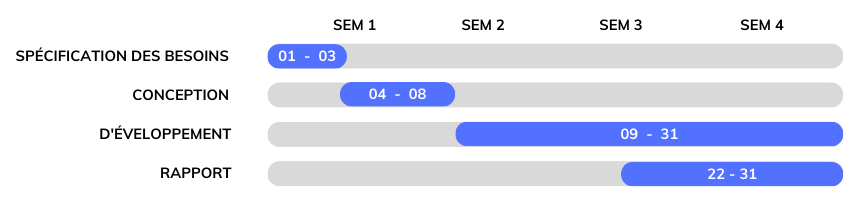
\includegraphics[scale=0.8]{gantt3}
  \caption{Diagramme de Gantt}
  \label{fig:votre-label}
\end{figure}
\section*{Conclusion}
\addcontentsline{toc}{section}{Conclusion}
A travers ce chapitre, nous avons clôturé notre projet en présentant des choix techniques. Nous avons exposé le travail effectué à travers les différentes interfaces apparues lors de l'exécution du projet.
\newpage
\section*{\begin{LARGE}
Conclusion générale et perspectives
\end{LARGE} }
\addcontentsline{toc}{section}{Conclusion générale et perspectives}
Ce projet de gestion des facturation développé au sein de l'Entreprise Tunisienne de l'Activité Pétrolière (ETAP) a été une opportunité exceptionnelle à plusieurs égards. Tout d'abord, il a marqué le début de mon parcours en tant qu'étudiant en génie logiciel à la Faculté des Sciences, en me permettant de mettre en pratique les connaissances et compétences acquises au cours de ma première année. En tant que projet d'initiation , il m'a ouvert les portes du monde professionnel de l'informatique, même si ce n'était que pour une courte période d'un mois.\\

En tant qu'étudiant en informatique, ce stage d'été a également été l'occasion d'explorer de nouvelles technologies et de renforcer mes compétences. J'ai eu la chance d'apprendre le langage SQL et de travailler avec MySQL pour gérer la base de données du projet. J'ai également plongé dans le monde de la conception logicielle en utilisant UML (Unified Modeling Language) pour modéliser l'architecture de l'application. De plus, j'ai découvert la bibliothèque Tkinter, une toute nouvelle expérience pour moi, en créant une interface utilisateur conviviale pour l'application. Mon expérience m'a également permis d'améliorer ma programmation en Python et d'apprendre à gérer un projet de développement de logiciel de A à Z.\\

En rétrospective, je considère que ce projet a été une étape importante dans mon parcours académique et professionnel. Bien que ma première année d'études ne m'ait pas encore exposé à de nombreux concepts avancés, j'ai abordé ce projet avec détermination et la volonté d'apprendre par moi-même. J'ai découvert la satisfaction de relever des défis techniques et de les surmonter grâce à l'auto-apprentissage.\\

En envisageant l'avenir de ce projet, je crois fermement qu'il existe des opportunités d'amélioration significatives. Une telle amélioration pourrait consister à intégrer la technologie OCR (Optical Character Recognition) afin de scanner automatiquement les factures, éliminant ainsi la saisie manuelle des données. Cette avancée serait une étape majeure vers l'automatisation complète du processus de gestion des factures, permettant ainsi de gagner du temps et d'accroître l'efficacité.

\end{document}
